% !TEX root = ../main.tex

\chapter{Experiments}
\label{chapter:Experiments}
The goal of our experimental evaluation is to understand how the two main ideas of our algorithm contribute to its 
performance in one observation, obscure goal POMDPs, namely the weak inductive bias as developed in \ref{COD_AC} and 
the inference time planning developed in \ref{inference_time_planning}. \\
To do this, we first analyze our weak inductive bias against a proposed method using a recurrent architecture.
We directly compare our results on the benchmark they provided. Second, we evaluate the performance difference between 
pure imitation learning and reinforcement learning with expert demonstrations on the reach environment from the Meta-World benchmark. 
Here we compare our inference time planning against two state of the arts reinforcement learning algorithms, which are pretrained using 
behavioural cloning. For our third experiment setup, we evaluate our approach against baselines on 5 tasks from the Meta-World benchmark. 
As one observation POMDPs are not well studied, we propose a variety of baselines aiming to challenge aspects we developed in our methodology.


\section{Imitation Learning}
In this section, we present our findings on the natural language conditioned robot manipulation task benchmark that was proposed by 
Simon Stepputtis et al. \cite{stepputtis2020languageconditioned}. The benchmark consists of a 7 dof simulated robot arm with a 
tabletop setup using CoppeliaSim, which allows for accurate dynamics simulations at an update rate of 20 Hz. The task is to pick 
up the correct cup and pour the content into the correct bowl, using natural language description of the cup and bowl and an RGB 
picture of the scene.\\

Three differently coloured cups containing a granular material that could be poured into the bowls were used. For the bowls, 
20 variations of two sizes, two shape types, and five colours were used. Successful picking action involved lifting a grasped 
object stably from the table, while successful pouring was detected whenever the cup's dispersed content ended up in the correct bowl. 
A random subset of objects was placed on the table, with a constraint to prevent collisions or other artefacts.\\

Figure \ref{lang_imi_expl} depicts the tabletop setup and the different variations of the objects used, as well as an example task.

As stated in appendix \ref{LCILRM}, in this experiment, only the first observation consisting of the RGB values from the picture of the 
scene and the task description is visible for the actor. With this setup, we want to evaluate our positional encoding bias. The method 
proposed in the accompanying paper "Language-Conditioned Imitation Learning for Robot Manipulation Tasks" uses a recurrent policy, which 
we will refer to as LCIL. As we have motivated in section \ref{COD_AC}, we expect our method to perform better than autoregressive or recurrent 
models because we use the knowledge that we are not getting additional information from the environment during the unroll of the trajectory. 
To test this, we have used the dataset of 40,000 expert demonstrations provided with the benchmark to train our model using only imitation learning.\\

The results are depicted in table

\begin{table}
    \centering
    \caption{Example table}
    \begin{tabular}{|c|c|c|}
        \cline{2-3}
        \multicolumn{1}{c|}{} & \textbf{Active Critic} & \textbf{LCIL} \\ \hline
        \textbf{Pick} & 100 \% & 98 \% \\ \hline
        \textbf{Pour} & 99 \% & 95 \% \\ \hline
        \textbf{Combined} & 98 \% & 92 \% \\ \hline
    \end{tabular}
    \caption{Success rates of the 100 pick, pour and combined tasks. The left column depicts the results from the Active Critic algorithm (ours) in 
    imitation mode. Right is the result of the LCIL architecture.}
\end{table}

On the 100 test environments that were provided, we decreased the overall error rate by 75$ \% $. 
\begin{figure}
    \captionsetup[subfigure]{justification=Centering, labelformat=empty}
    \begin{subfigure}[t]{0.18\textwidth}
        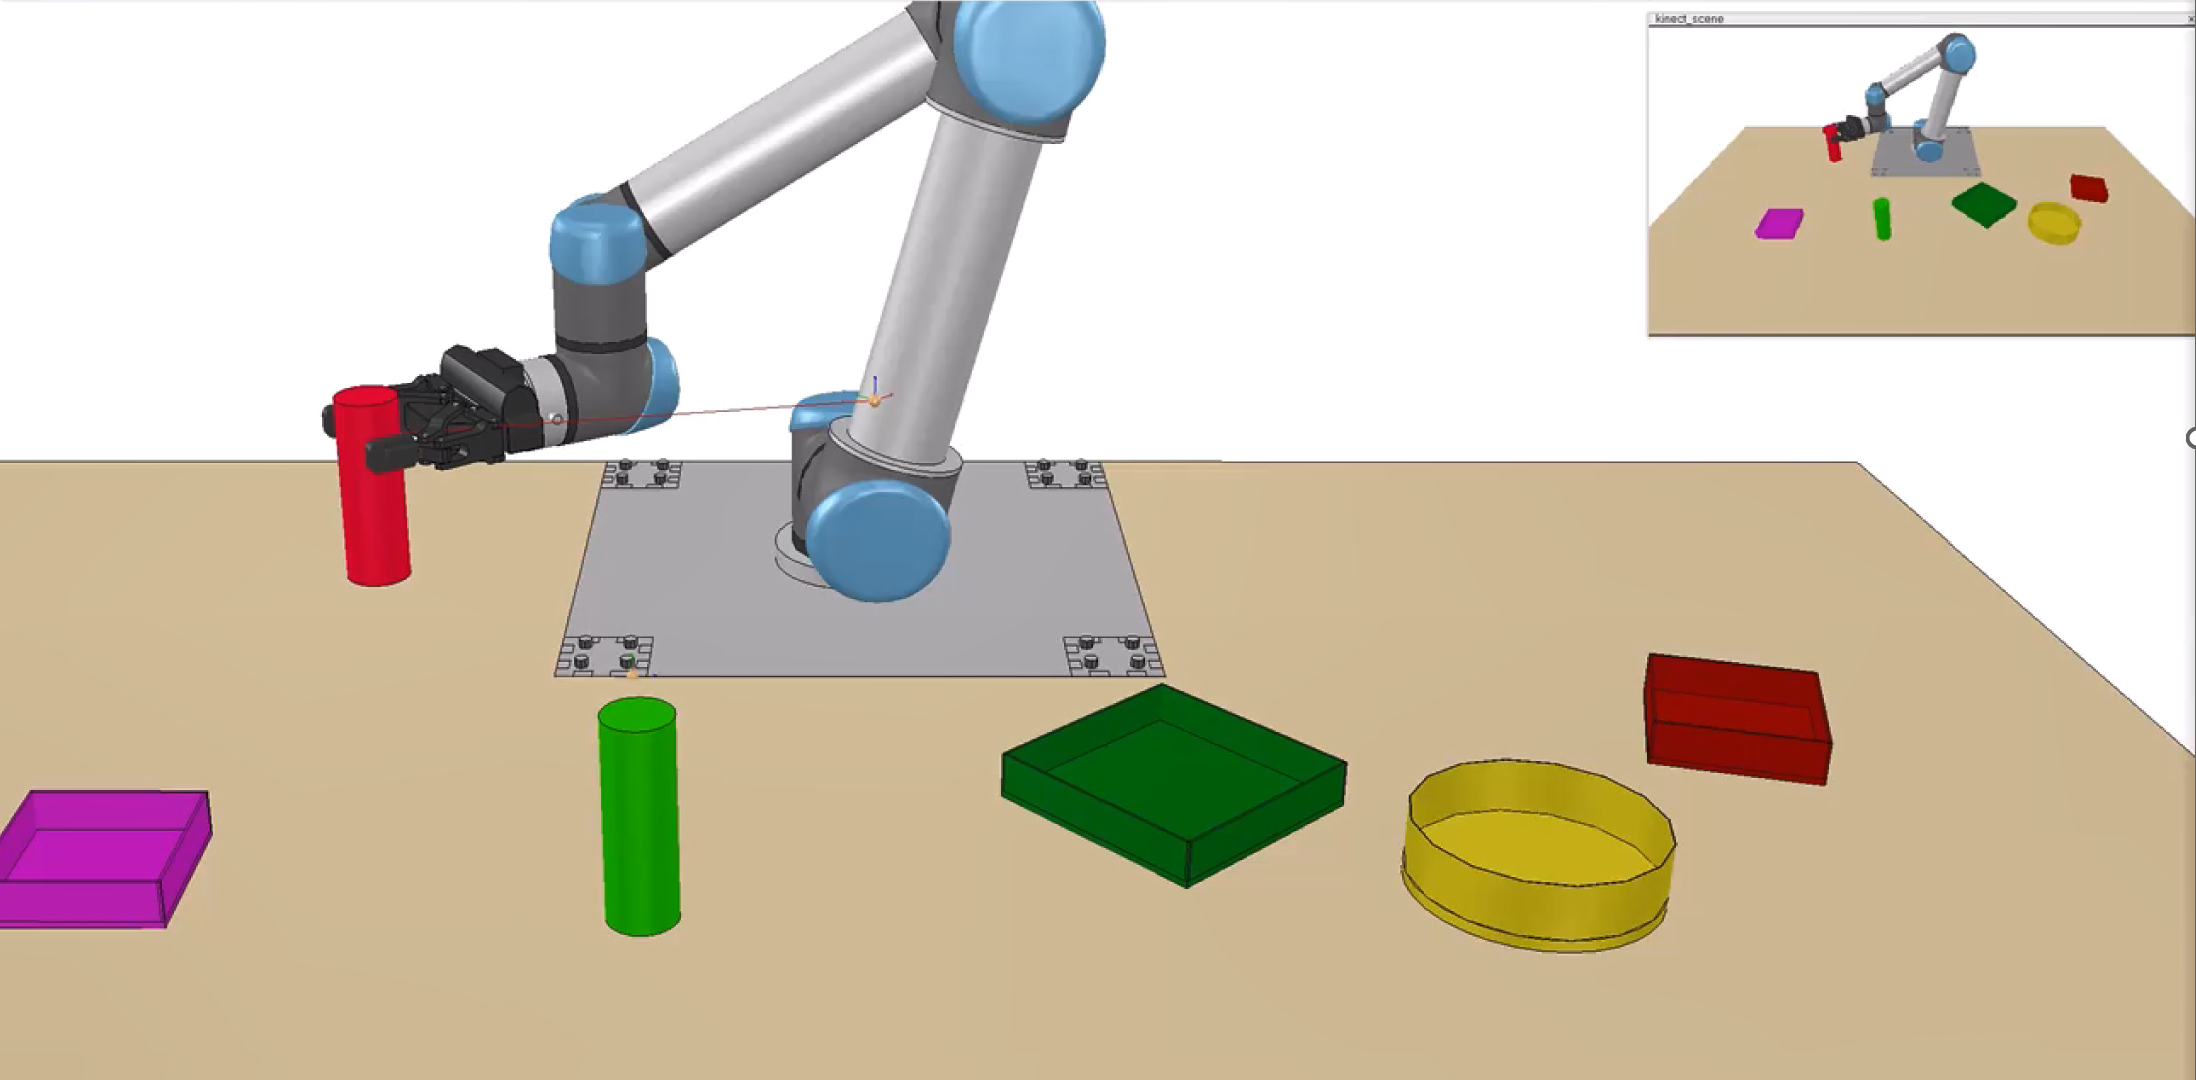
\includegraphics[width=\textwidth]{images/Language_Conditioned_Exp/theirs_1.png}
        \caption{Time step 60.}
    \end{subfigure}
    \begin{subfigure}[t]{0.18\textwidth}
        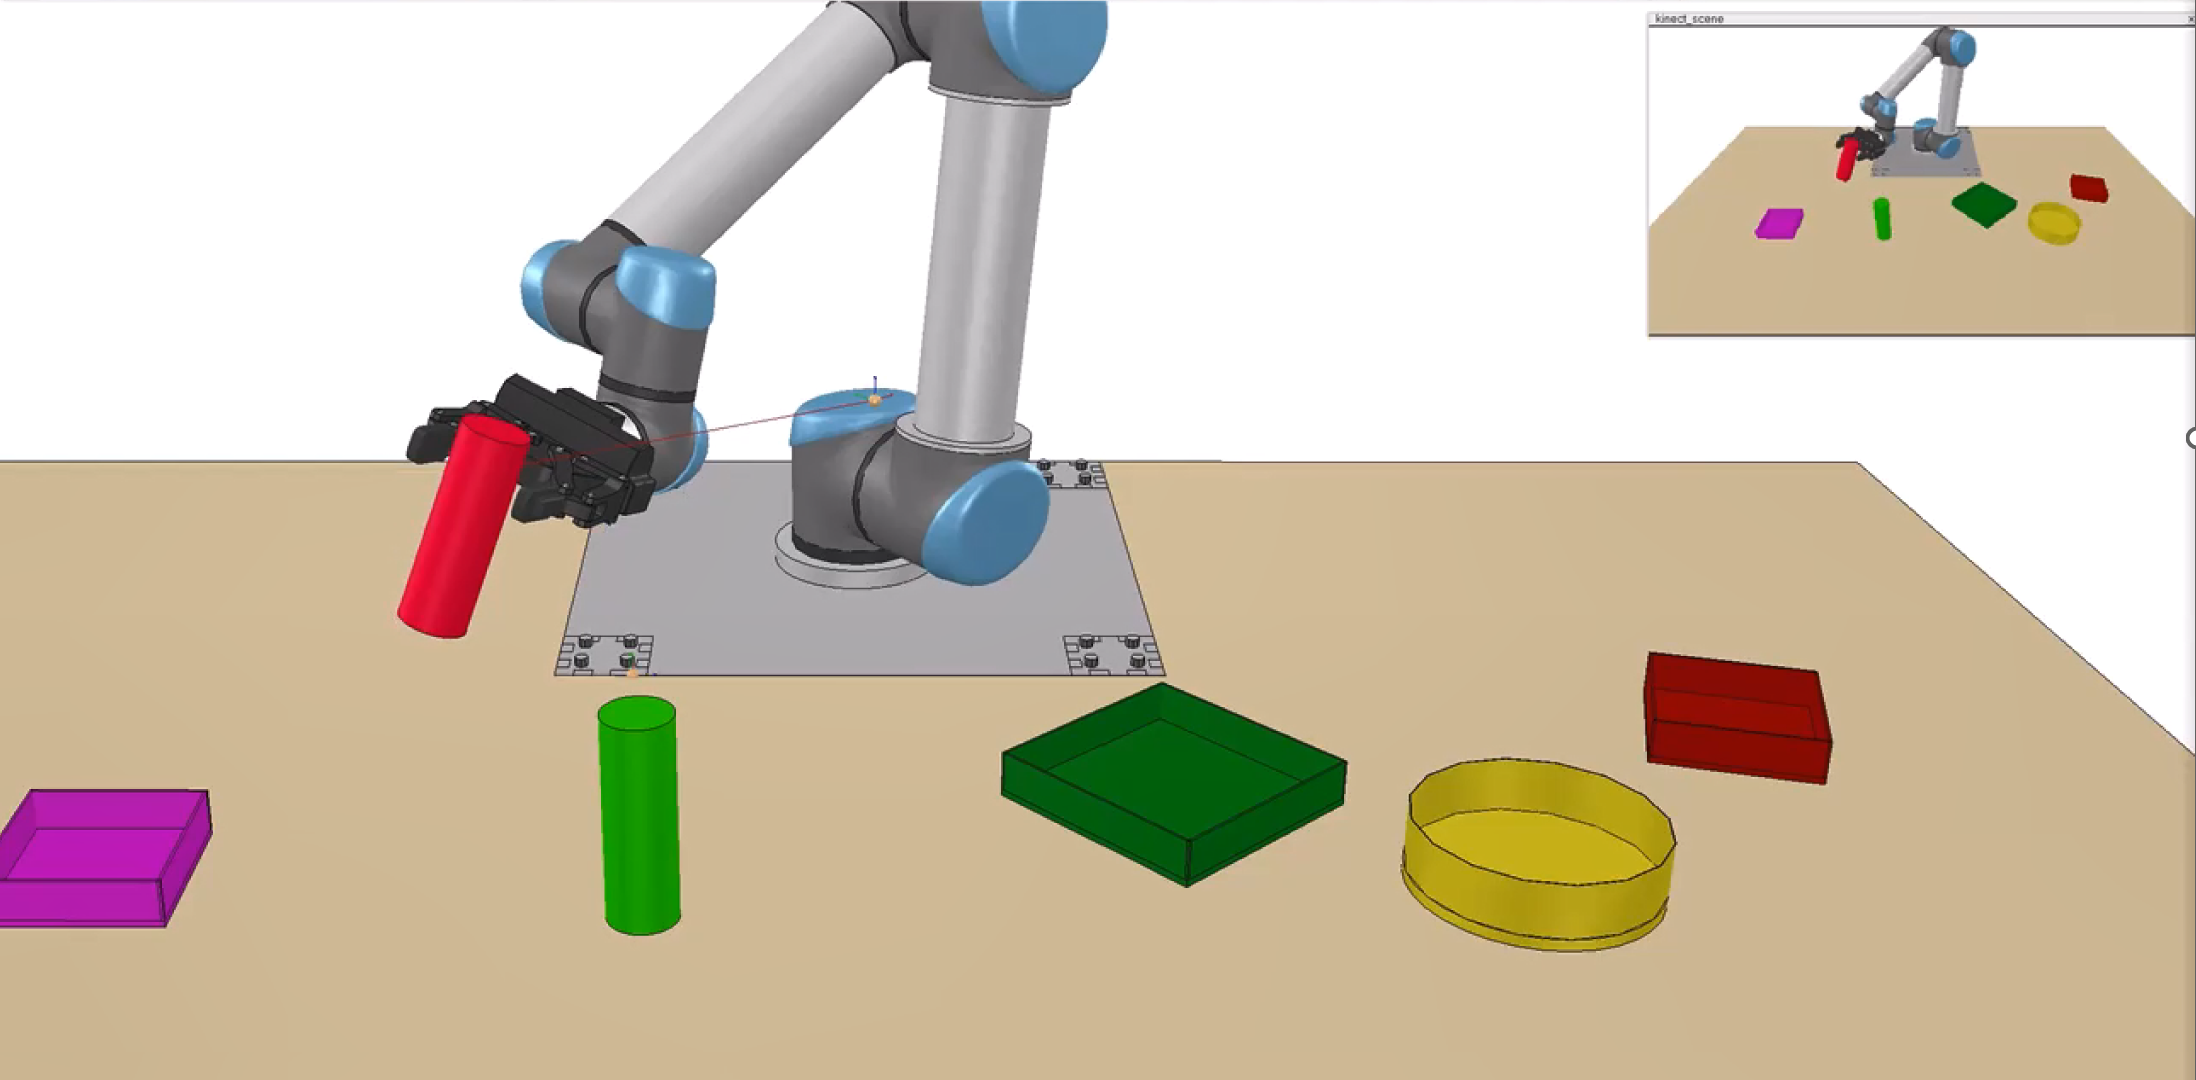
\includegraphics[width=\linewidth]{images/Language_Conditioned_Exp/theirs_2.png}
        \caption{Time step 120.}
    \end{subfigure}
    \begin{subfigure}[t]{0.18\textwidth}
        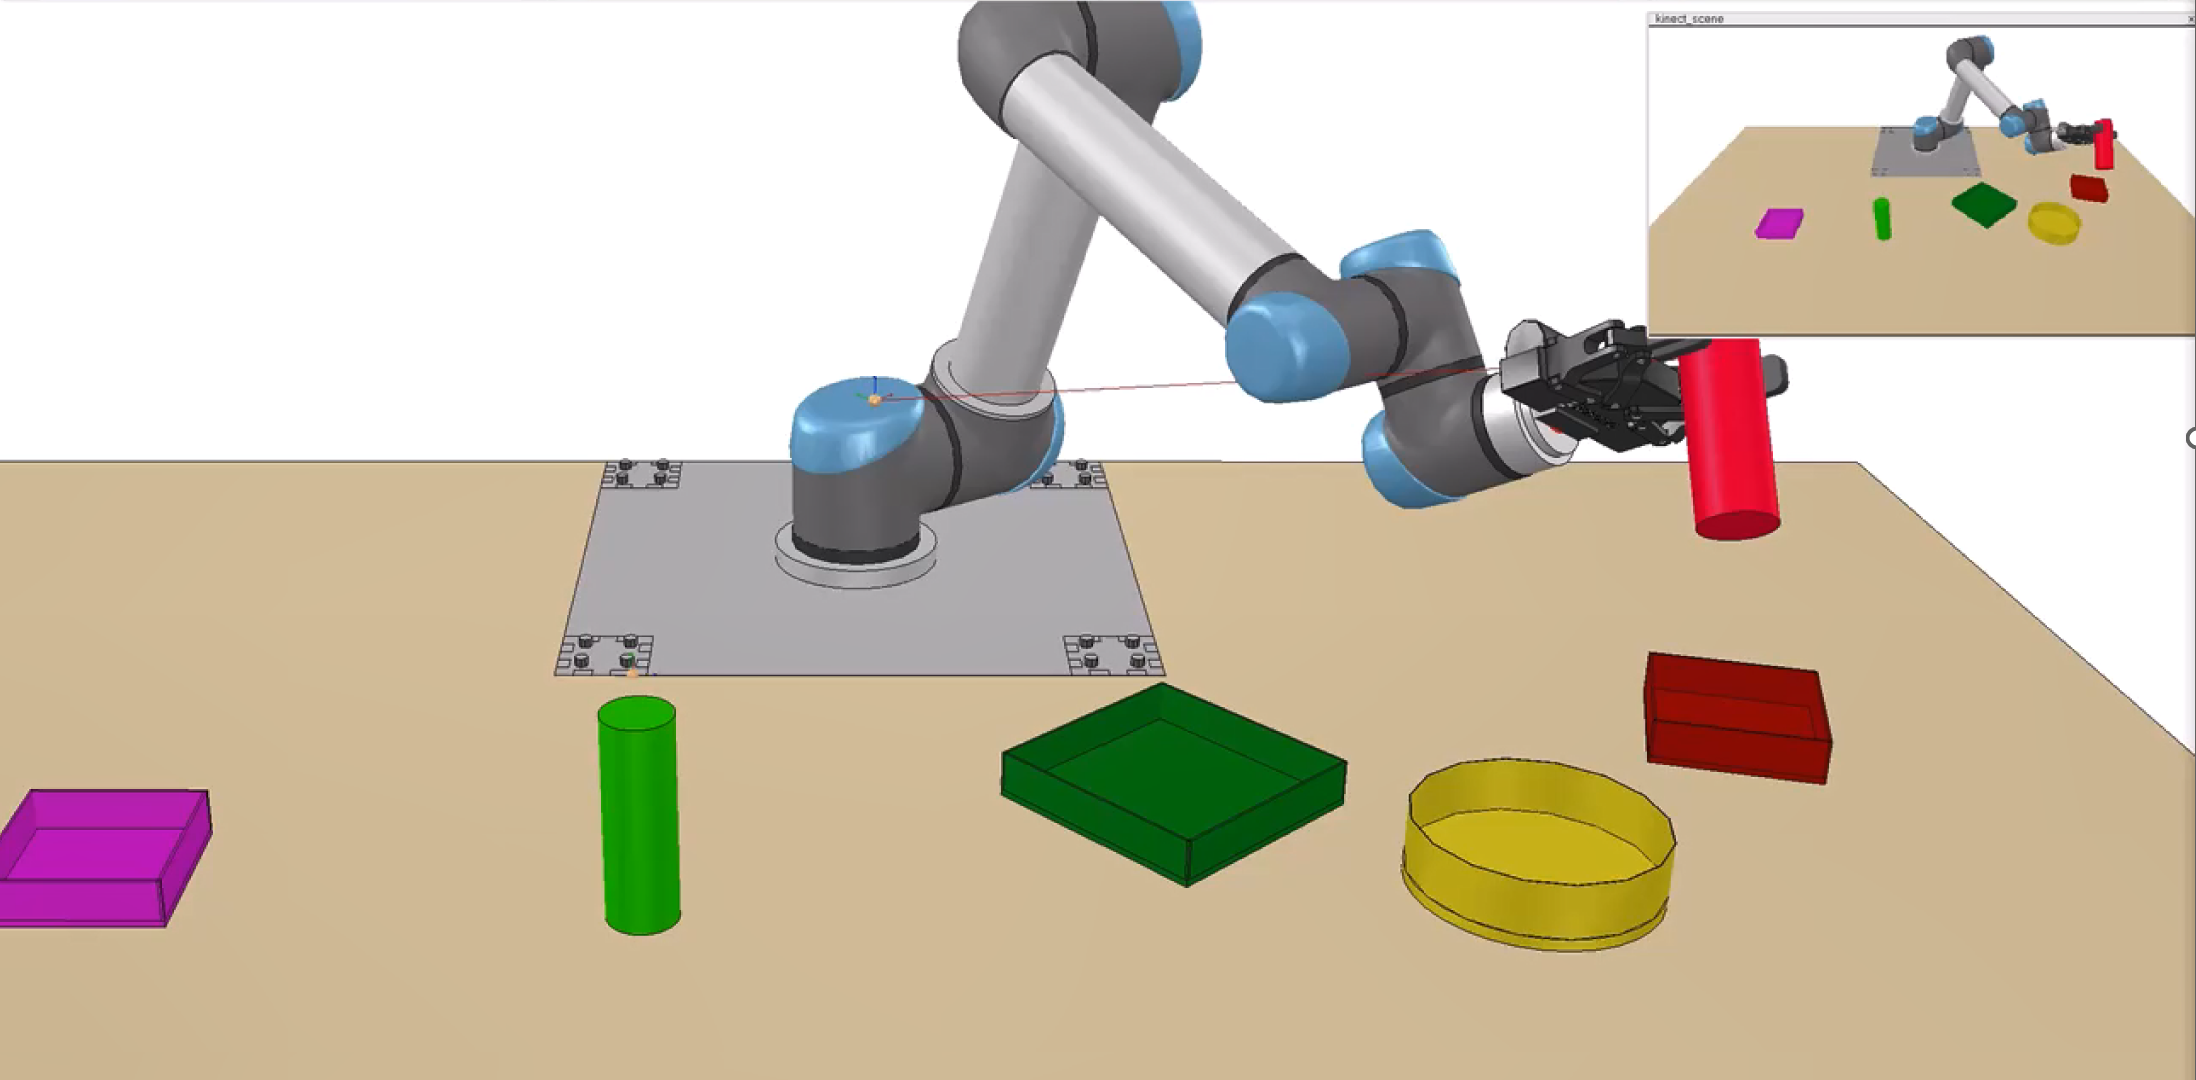
\includegraphics[width=\linewidth]{images/Language_Conditioned_Exp/theirs_3.png}
        \caption{Time step 180.}
    \end{subfigure}
    \begin{subfigure}[t]{0.18\textwidth}
        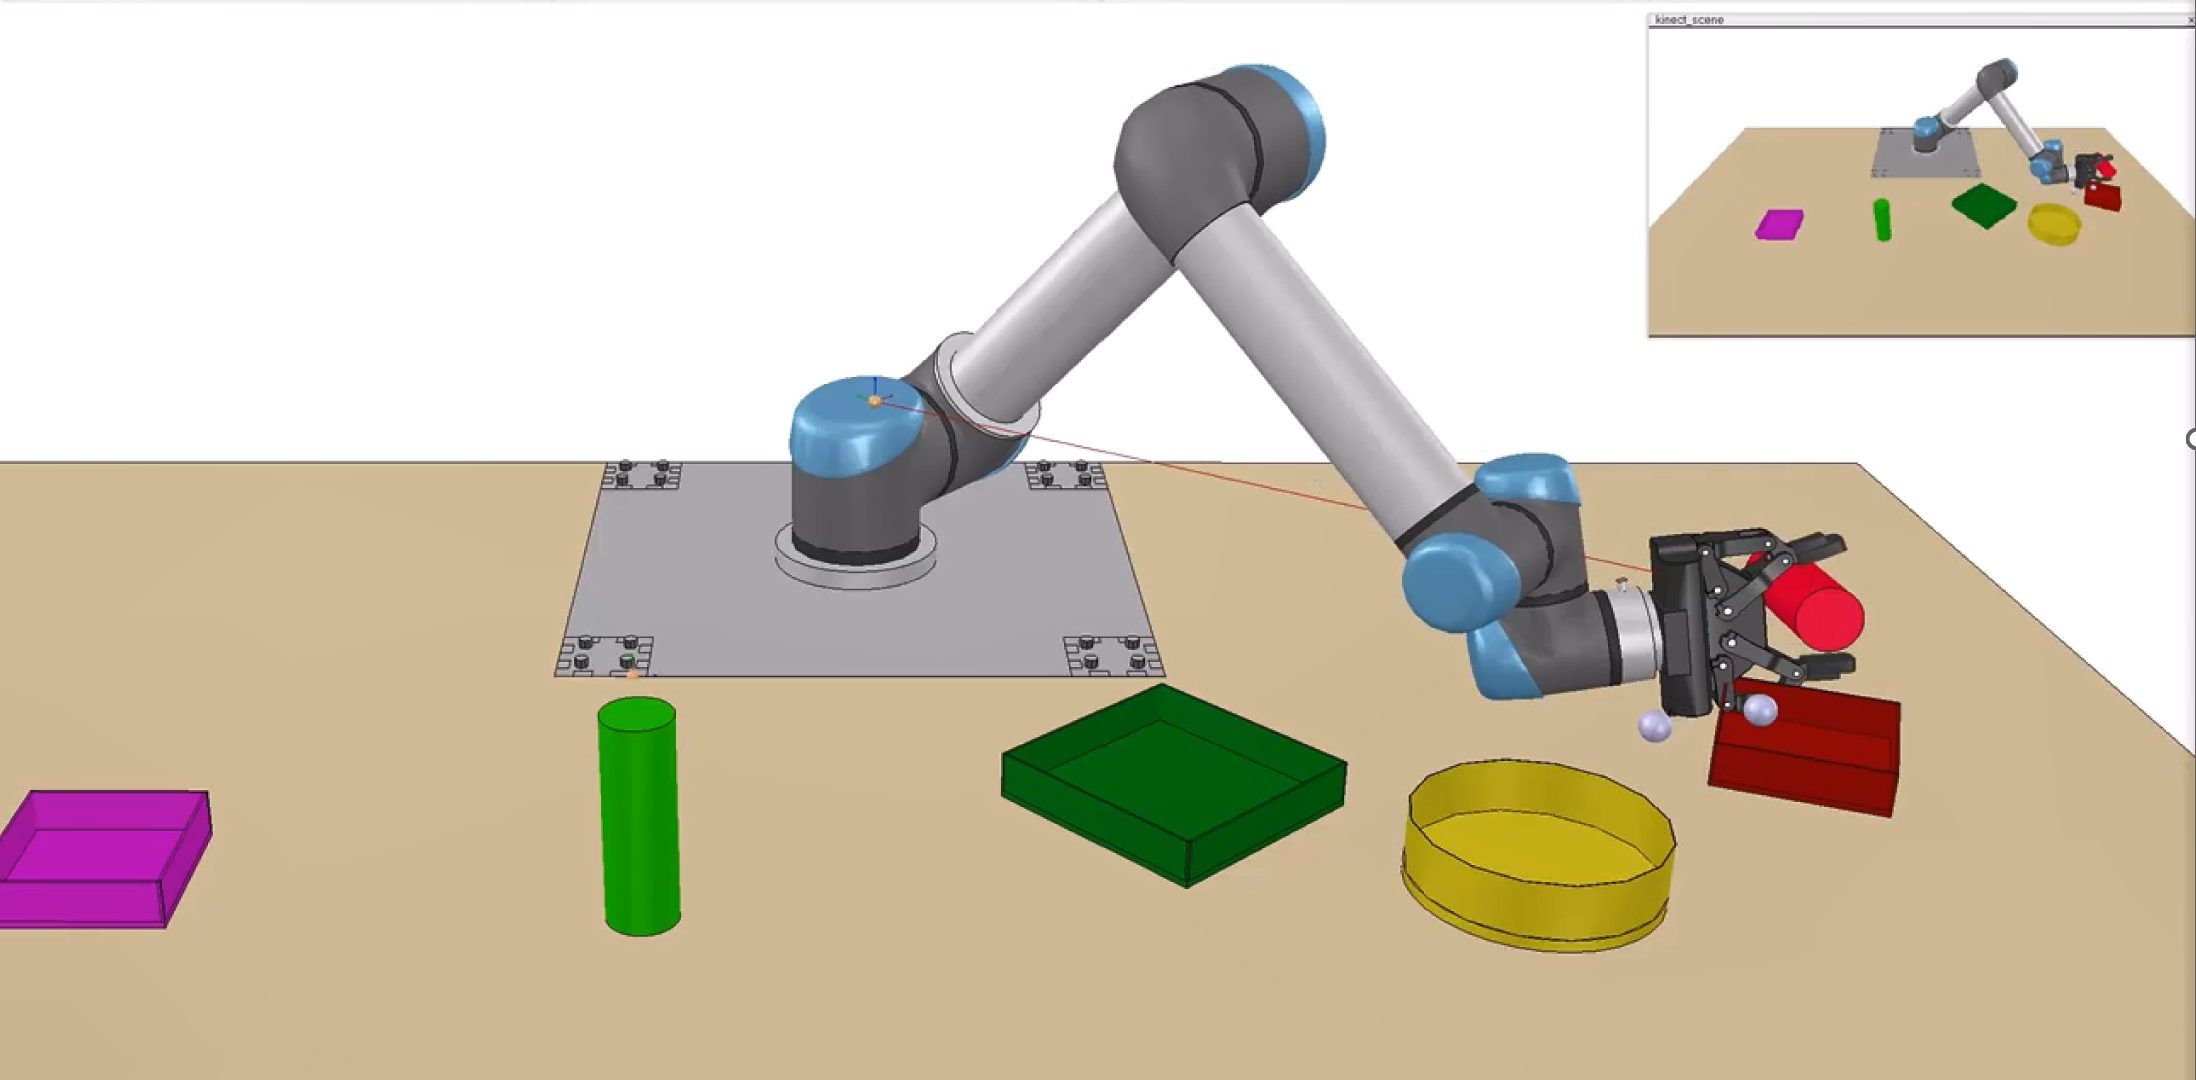
\includegraphics[width=\linewidth]{images/Language_Conditioned_Exp/theirs_4.png}
        \caption{Time step 240.}
    \end{subfigure}
    \begin{subfigure}[t]{0.18\textwidth}
        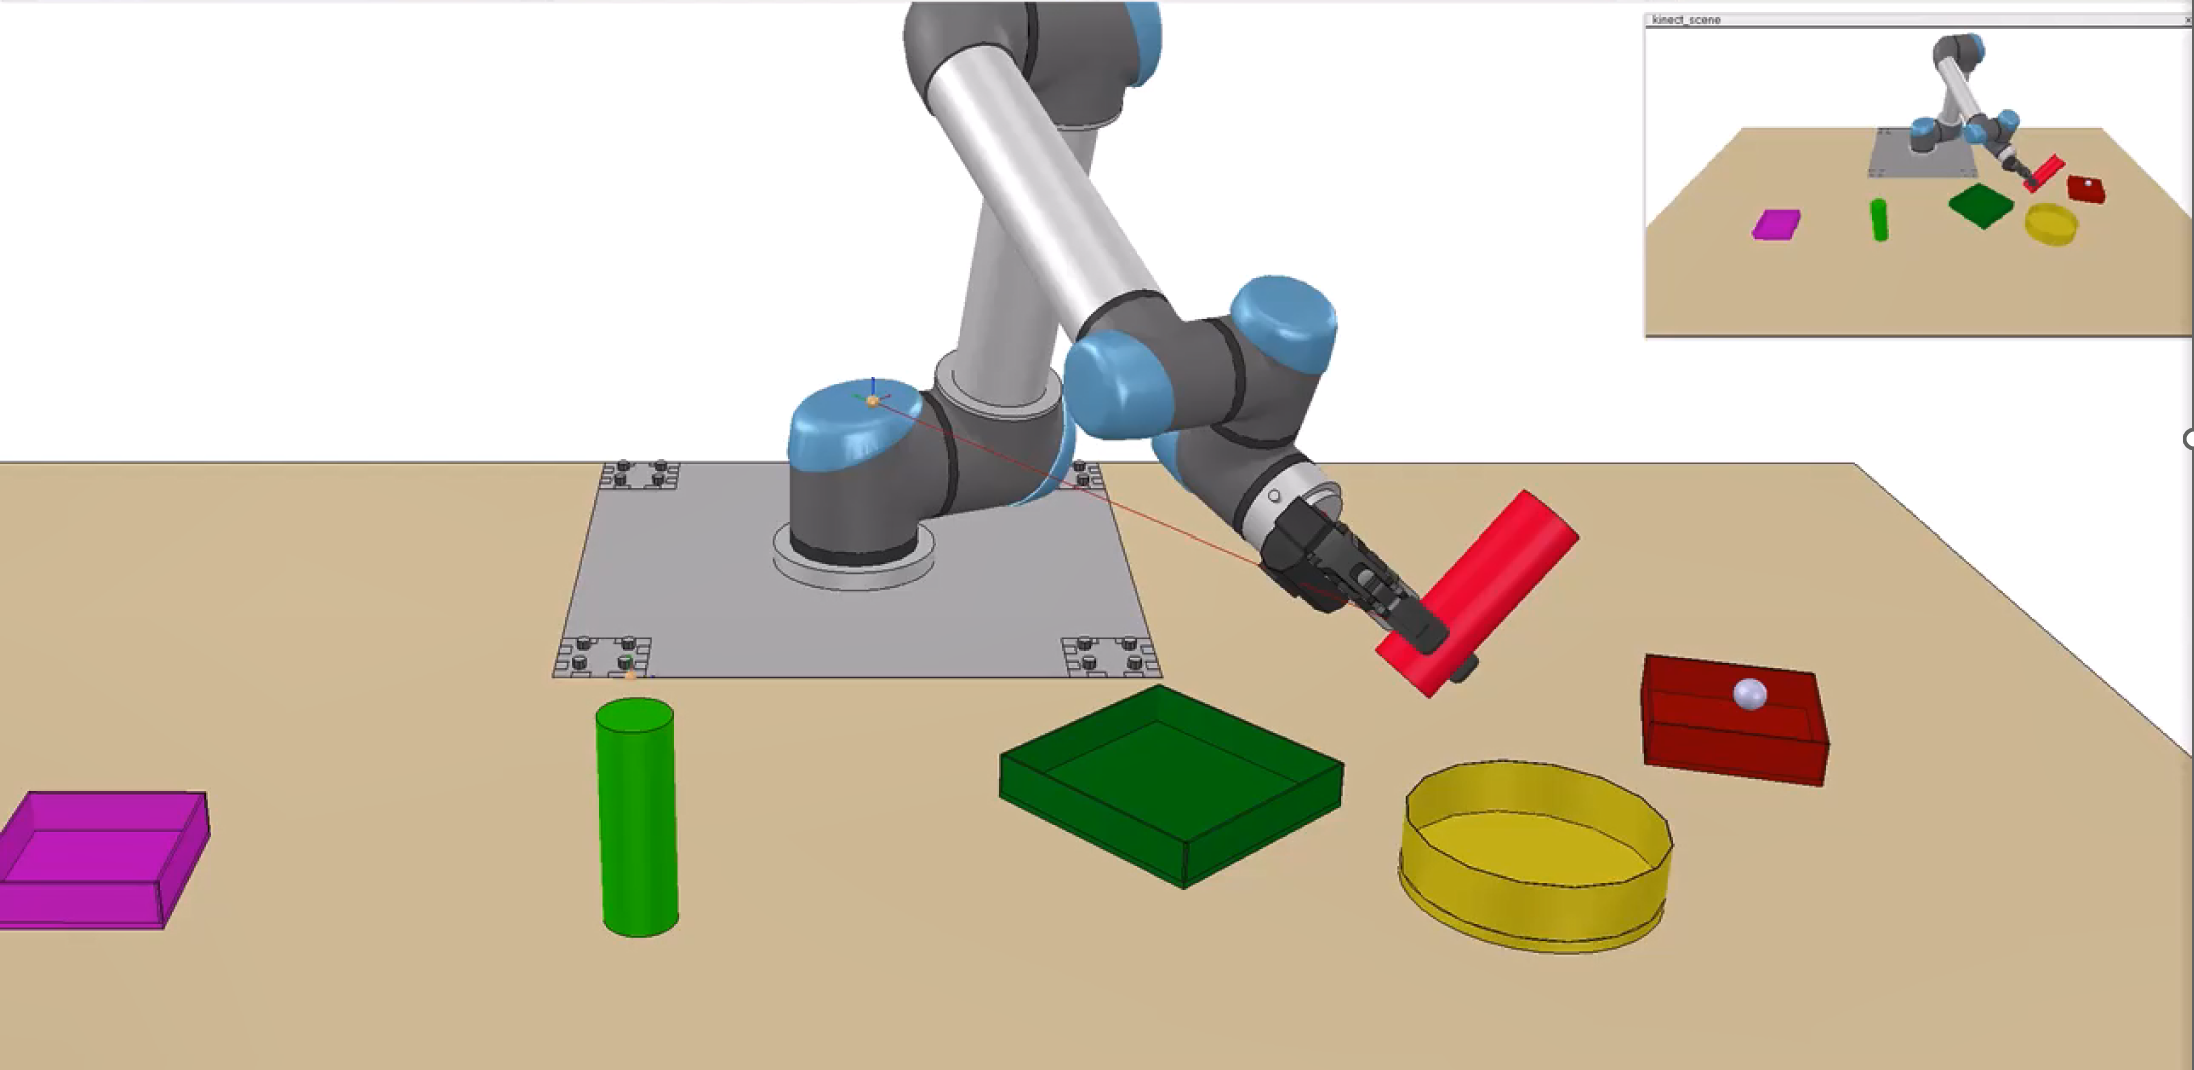
\includegraphics[width=\linewidth]{images/Language_Conditioned_Exp/theirs_5.png}
        \caption{Time step 300.}
    \end{subfigure}

    \bigskip % more vertical separation
    \begin{subfigure}[t]{0.18\textwidth}
        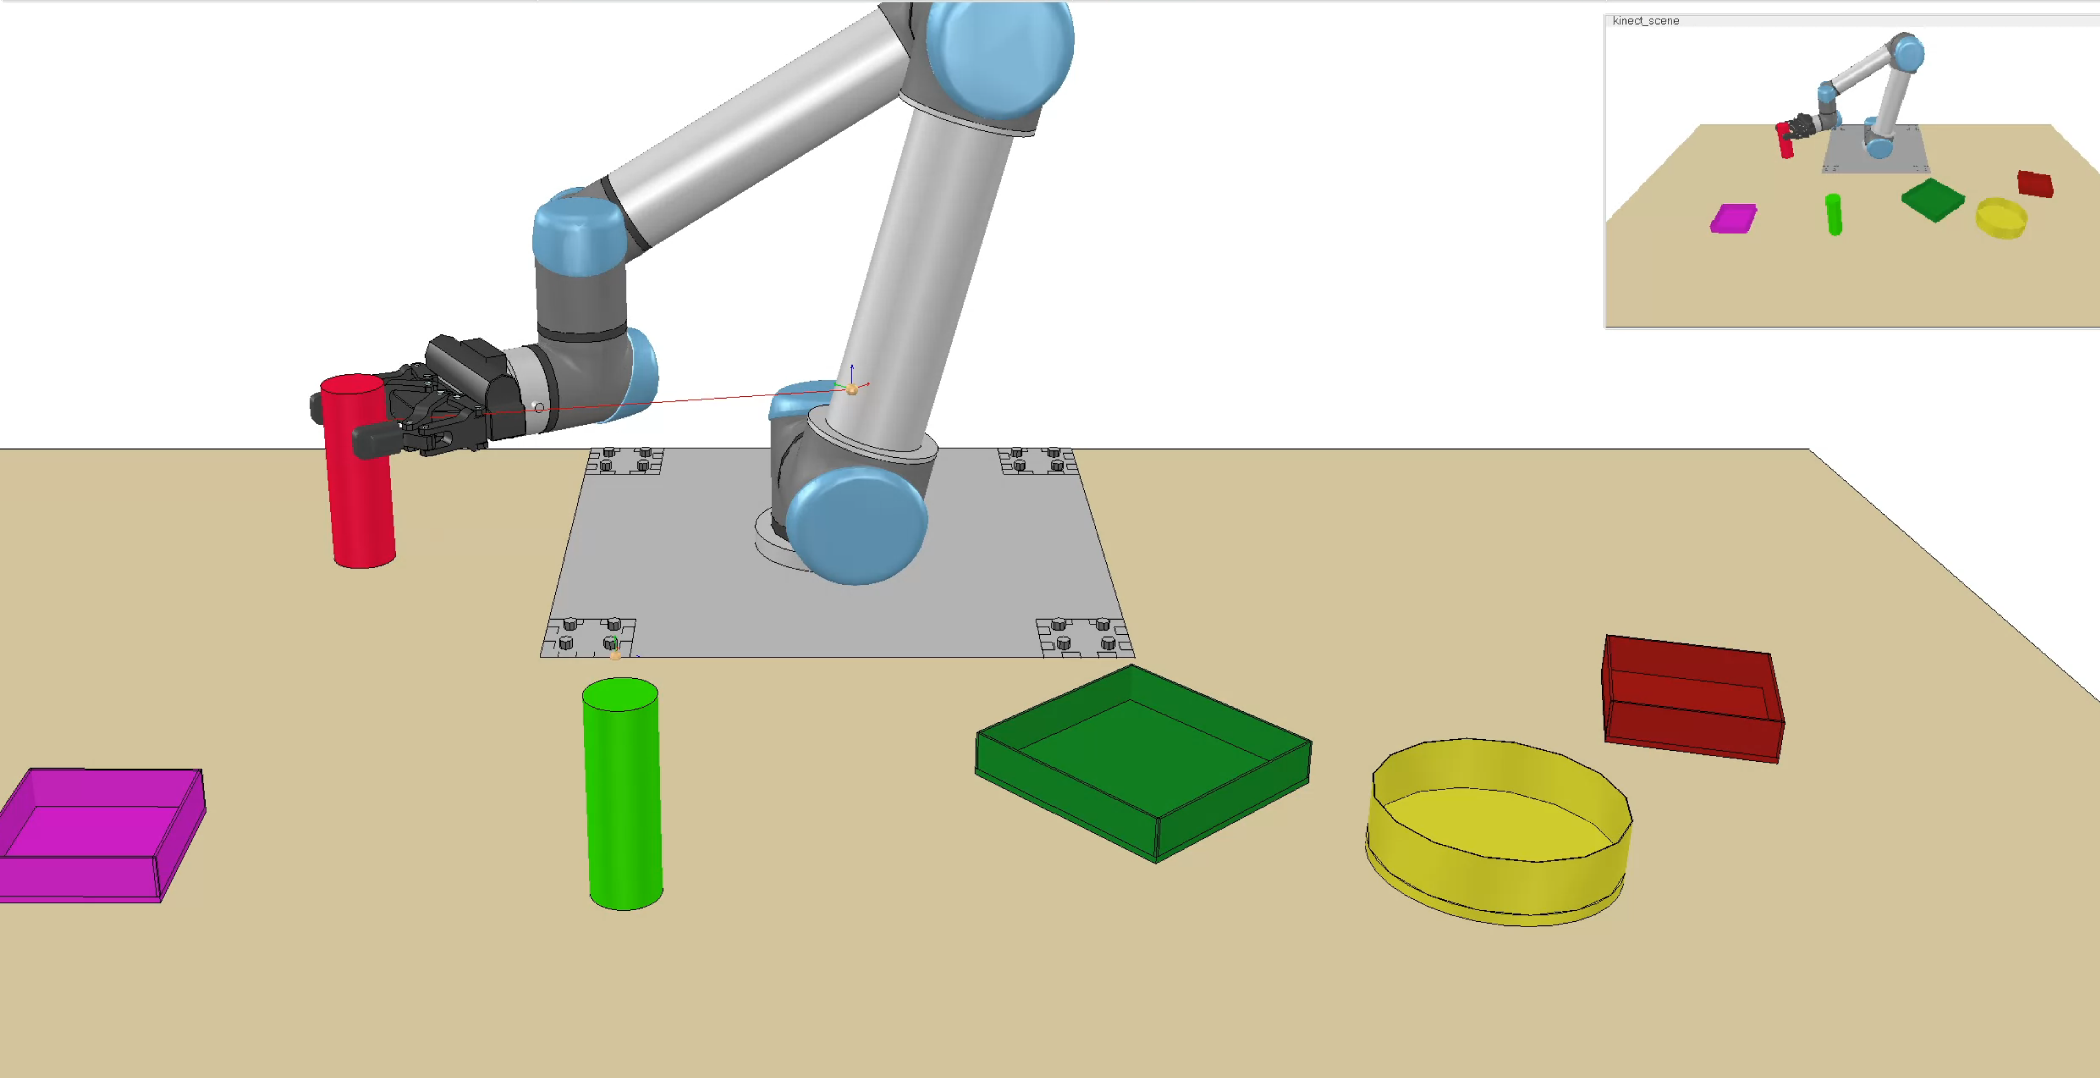
\includegraphics[width=\linewidth]{images/Language_Conditioned_Exp/mine_1.png}
        \caption{Time step 60.}
    \end{subfigure}
    \begin{subfigure}[t]{0.18\textwidth}
        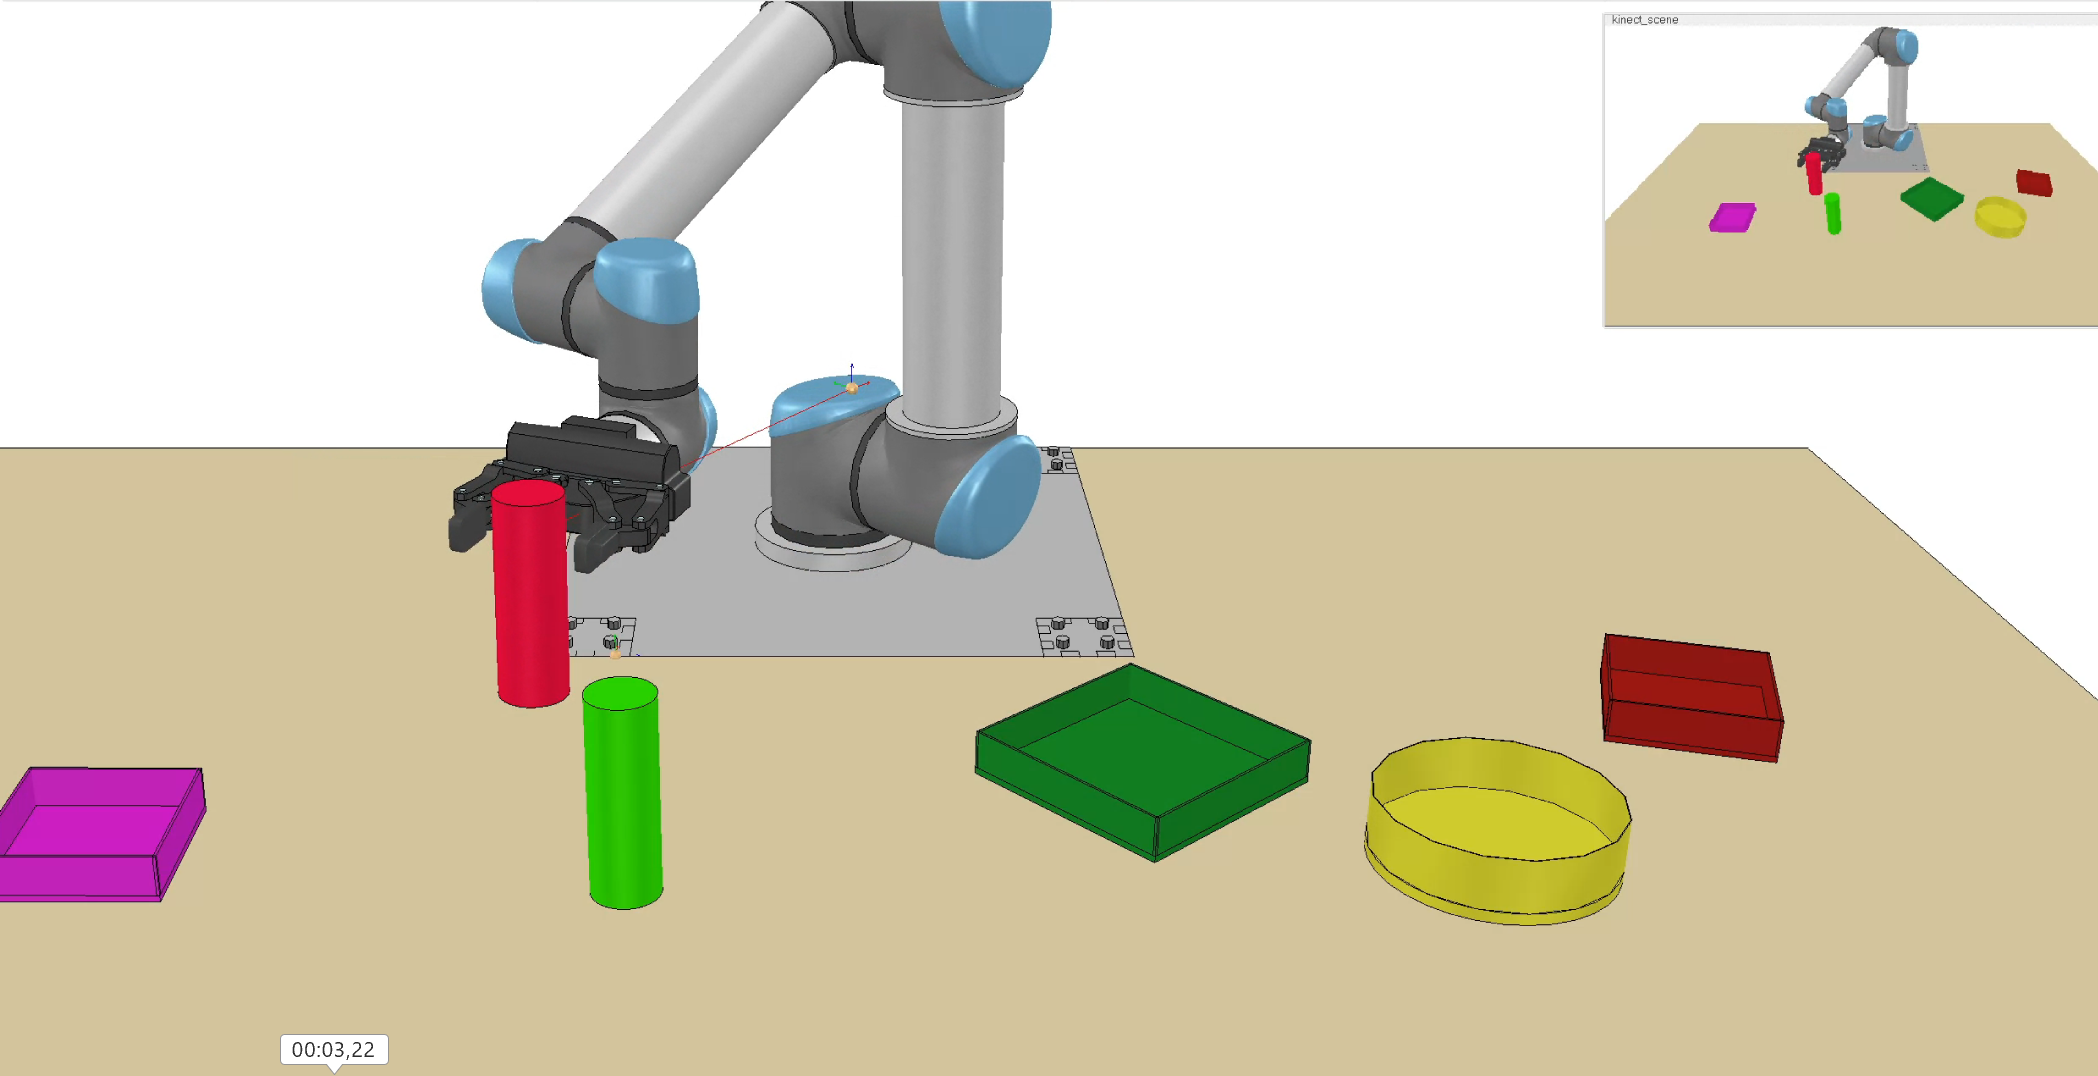
\includegraphics[width=\linewidth]{images/Language_Conditioned_Exp/mine_2.png}
        \caption{Time step 120.}
    \end{subfigure}
    \begin{subfigure}[t]{0.18\textwidth}
        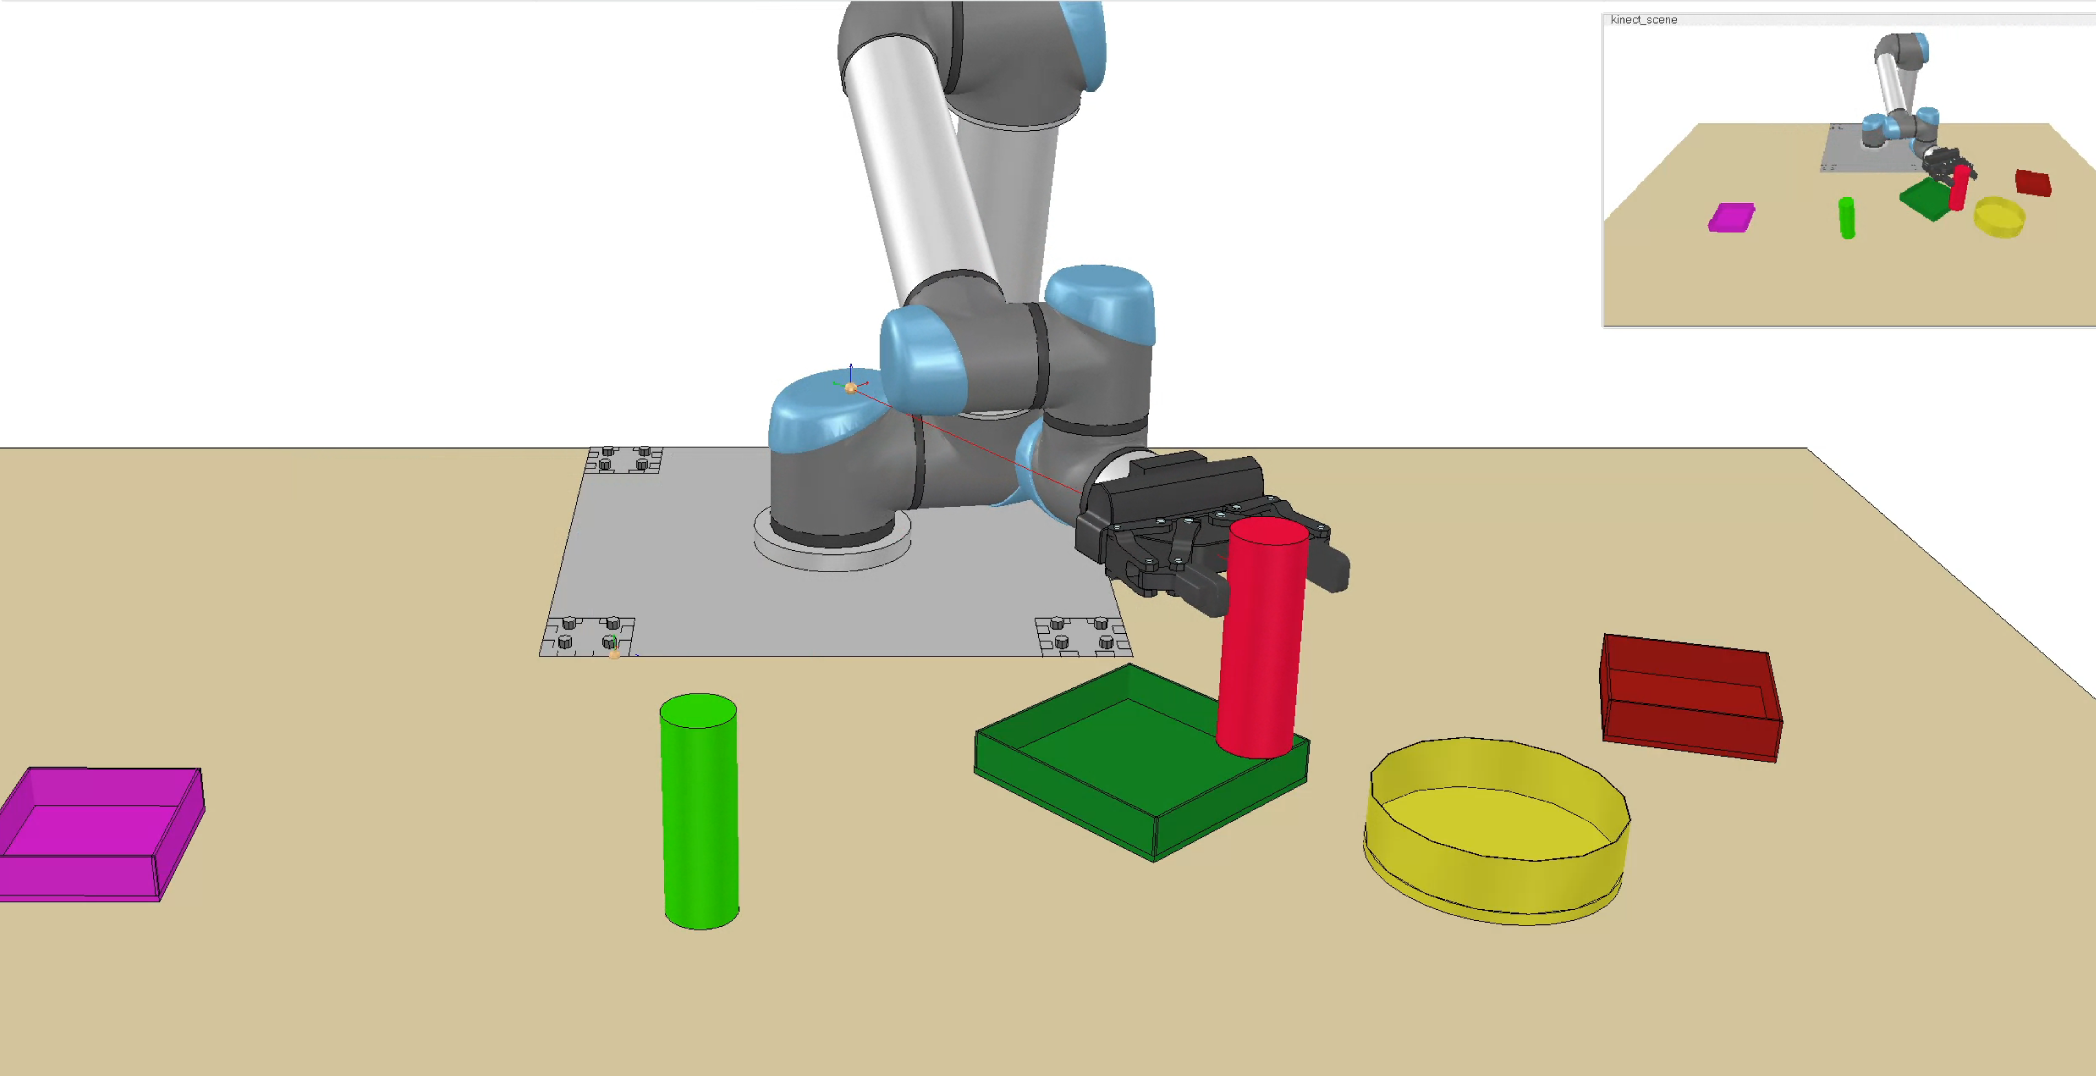
\includegraphics[width=\linewidth]{images/Language_Conditioned_Exp/mine_3.png}
        \caption{Time step 180.}
    \end{subfigure}
    \begin{subfigure}[t]{0.18\textwidth}
        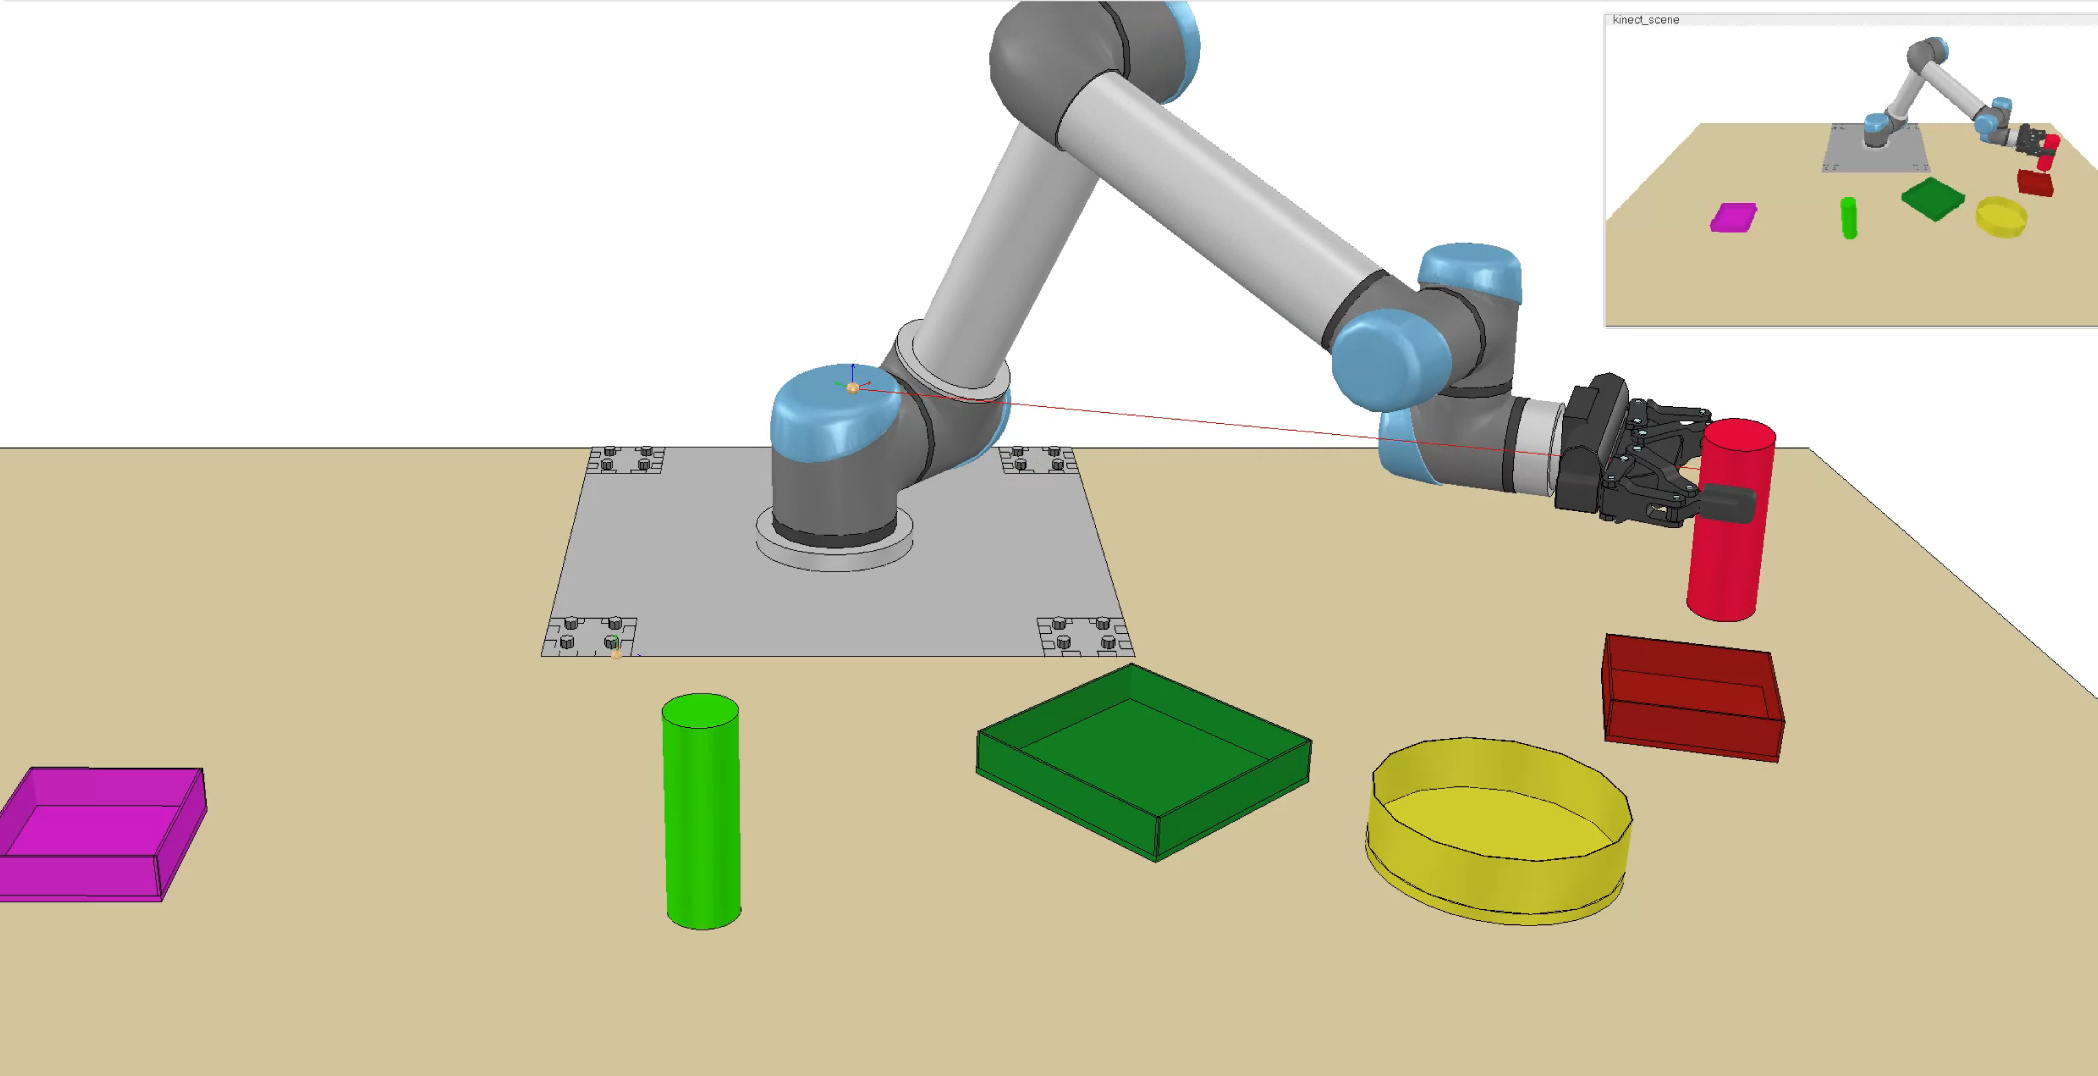
\includegraphics[width=\linewidth]{images/Language_Conditioned_Exp/mine_4.png}
        \caption{Time step 240.}
    \end{subfigure}
    \begin{subfigure}[t]{0.18\textwidth}
        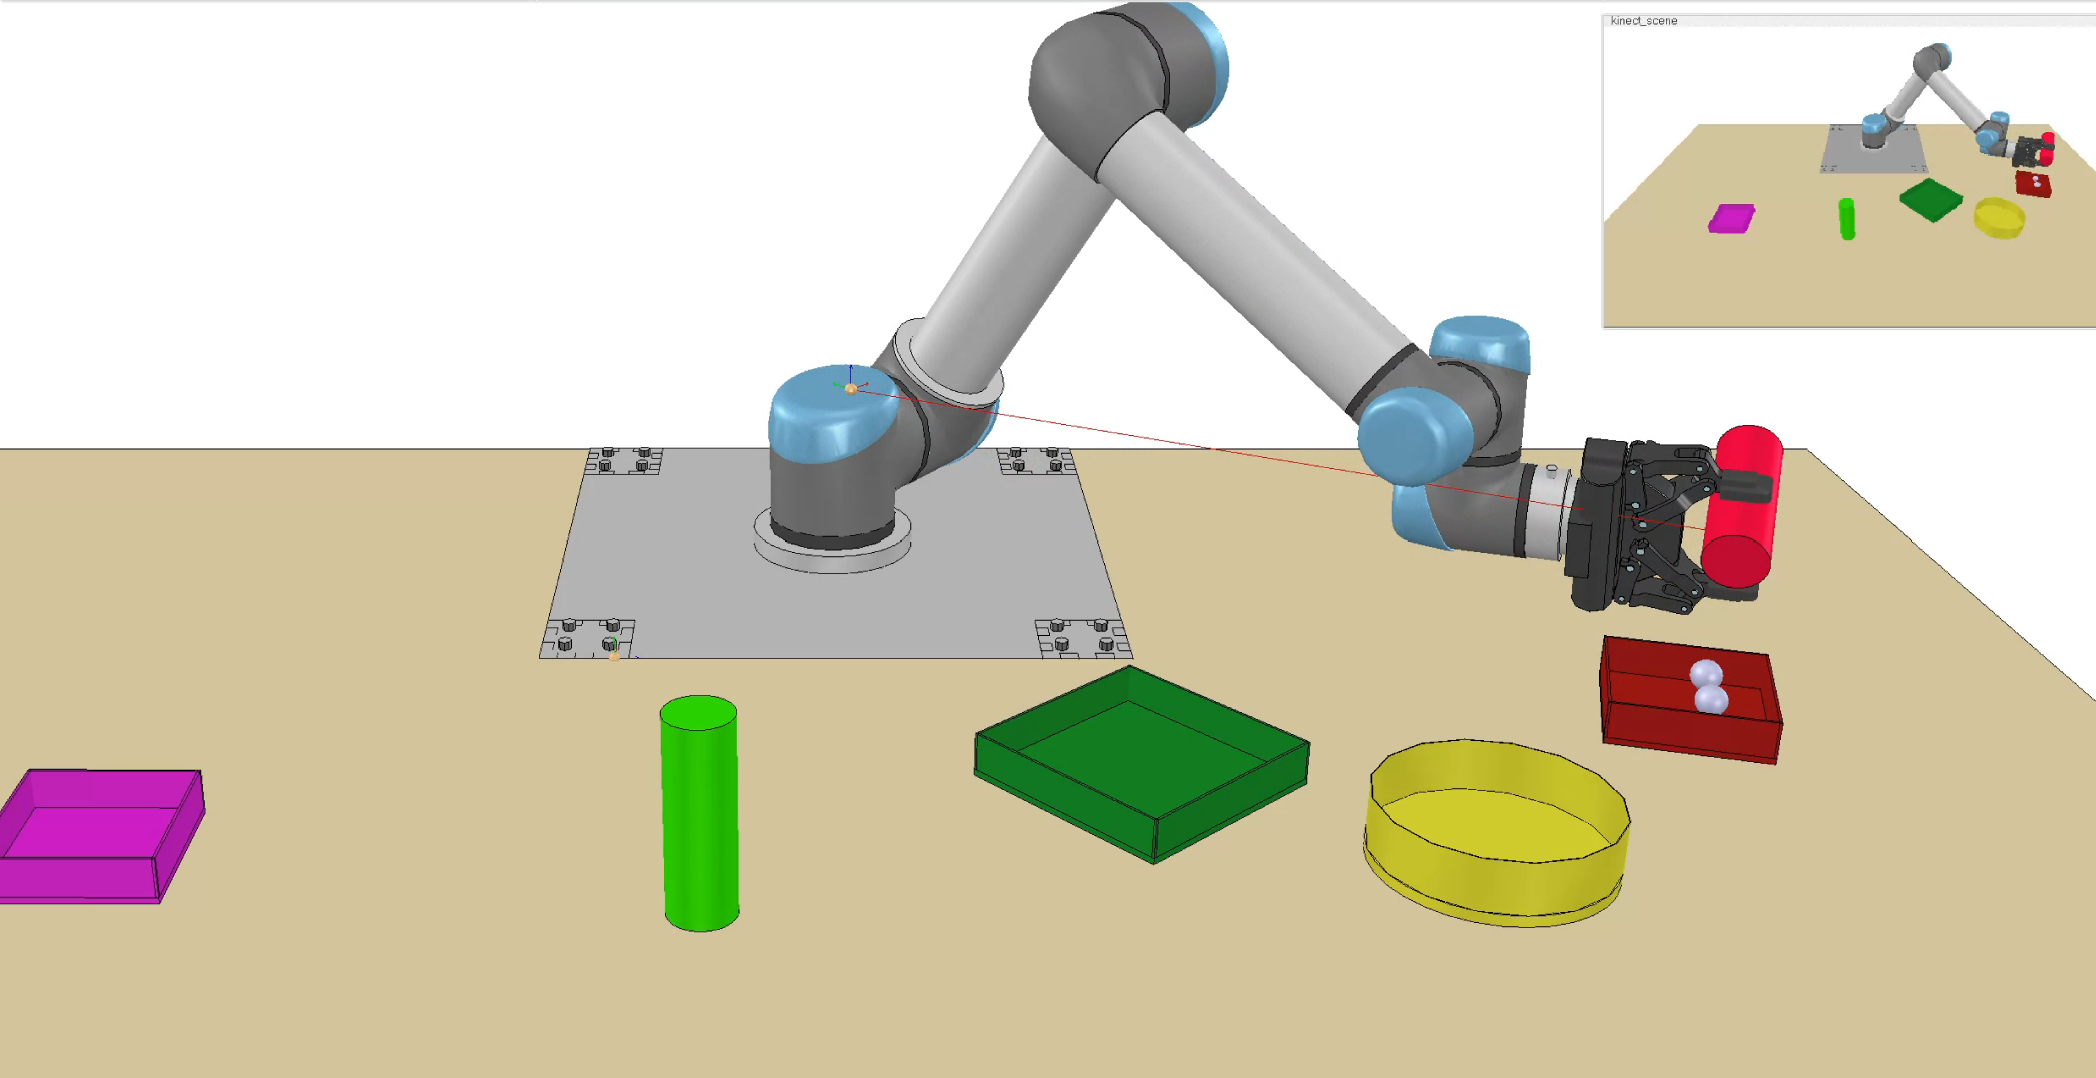
\includegraphics[width=\linewidth]{images/Language_Conditioned_Exp/mine_5.png}
        \caption{Time step 300.}
    \end{subfigure}
    \caption{Comparison of a pour task. The policy learned by the LCIL algorithm (top row) spills the content over the table and moves unpredictable. The task is considered a failure 
    by the benchmark, as most drops did not land in the goal bowl. Active Critic (bottom row) performs the task as intendet with no unexpected movement.}
    \label{fig: AVC vs. Rec}
\end{figure}
Furthermore, in Figure \ref{fig: AVC vs. Rec}, we have depicted a case in the test dataset that our policy solved and compared it to the performance 
of the recurrent algorithm, which failed at the task.
While our approach hit the target precisely, the recurrent model was widely off. We assume that this is caused by the fact that during inference 
time, the
i.i.d. assumption of the input data to the policy is broken. Intuitively, the recurrent policy
is in a state that it has not seen before and acts slightly differently to the expert movement. After some steps, the policy now sees 
inputs that are vastly
different from the training distribution, thus it starts to act unpredictably. As argued in Section \ref{COD_AC}, this is an advantage of our 
policy as it
does not break the i.i.d. assumption.

\section{Reinforcement Learning from Sparse Rewards in Single Observation Environments}
In this section, we will explore the performance of the AVC algorithm given a single observation per trajectory, one sparse reward per trajectory, and some expert demonstrations.
We motivated the practical relevance in the introduction. An additional advantage for testing the effectiveness of the search paradigm is that planning is most efficient in
single observation settings.
We discussed this in section \ref{sec:AC_Critic}, where we state that while predicting the MDP has a quadratic error bound, we don't get any updated information
during the trajectory, and thus no better estimate is possible. \\

We chose environments from the "Meta-World" \ref{yu2019meta} benchmark, as they have a success indication per environment, from which sparse rewards can be defined naturally.
Specifically, we chose five environments from the ML10 suite, namely "Pick and Place", "Push", "Reach", "Window Open" and "Drawer Close", which represent a variety
of difficulty levels suited to test different aspects of our algorithm. We defined a constant sequence length of 100 steps per trajectory and provided
a reward at the end according to whether the environment was solved at any step along the trajectory. Additionally, the environment
only returns the initial observation along the trajectory.\\

The single observation setup is not well-studied in continuous spaces, so we have to find baselines that are best suited to challenge the performance of our algorithm. For sparse rewards, a common
algorithm is "HER" as discussed in section \ref{sec:HER}, but it assumes a way to compute the goal from an environment state. This is not suitable in our setup, as we don't have access to the environment
states after the first state. Moreover, this assumption limits the generality of the approach, which AVC does not need to.
We use PPO, a state-of-the-art on-policy algorithm, and TQC, a state-of-the-art off-policy algorithm, together with transformer-style sequential encoding to indicate the timestep. We also include
RPPO, a recurrent implementation of PPO, where we repeatedly input the initial observation and use the hidden states to encode the position along the action sequence.
PPO, TQC, and RPPO were pre-trained using behavioural cloning. We chose the best-performing policy during behavioural cloning by testing the policy on 50 test
trajectories every 400 full cycles through the
expert transitions. Technically, these test trajectories were environment interactions, but we chose not to count them to give the best-case comparison to the AVC algorithm, which was not pre-trained.\

For the base implementations, we use "Stable Baselines3" \ref{stable-baselines3}, which is a common choice, as it provides well-implemented algorithms with tested
performance and fine-tuned hyperparameters for a wide range of environments. This includes our chosen environments, but with dense rewards and continuous observations,
thus some hyperparameter tuning was necessary. \\

In the following sections, we will test our algorithm in two different settings, namely fine-tuning and guided reinforcement learning. In fine-tuning, we provide
enough expert demonstrations, that the environment can be solved with acceptable performance, but with room for improvement. In guided reinforcement learning,
only one expert demonstration is provided. AVC will use the same set of hyperparameters for all experiments to showcase its generality and robustness. Also, we had no choice for time constraints.
We will use limited fine-tuning for the baselines, however.
With these experiments, we aim to test both exploitation and exploration of our algorithm and show stable
behaviour across a wide range of use cases. \\

In all plots, the first data point is sampled from the policy before any environment interaction. For the plots with behavioural cloning, it indicates learned performance from expert trajectories.
In plots with no provided expert trajectory, it displays the behaviour following random initialization.


\subsection{Fine Tuning}
\label{sec:fine_tuning}
In this section, we analyse our algorithm in a fine-tuning setup. We provided the algorithms with 4 and 15 expert demonstrations per 
environment and used a relatively short reinforcement learning phase with 400 sampled trajectories consisting of 100 steps each. We 
repeated each experiment four times with 30 test trajectories per datapoint. One problem we wanted to overcome is "catastrophic forgetting" 
that can occur when the data distribution shifts. During the imitation phase, the learners only see positive examples sampled according to 
the distribution induced by the expert, which leads to overestimation by the critic. Our algorithm is more robust to this problem, as it 
decouples the actor from the critic, as discussed in section \ref{inference_time_planning}. We present our findings in figure \ref{fig:finetuning}. 
For the environments "Pick and Place" and "Push", we show the plots for 15 expert demonstrations, as we found 4 expert demonstrations were not 
enough to meaningfully learn within 400 training episodes. The environments "Reach" and "Window Open" are easier to learn, so we display the 
experiments with 4 expert demonstrations each, as giving 15 expert demonstrations lead to near perfect performance from imitation learning alone. 
All plots for all experiments can be found in Appendix \ref{chapter:additional_plots}.\\

We expected RPPO to be the least performant from our discussion of the curse of dimensionality in section \ref{COD_AC}. As no current input 
is provided from the environment, RPPO has to keep track of all previous actions. PPO and TQC use positional encoding to indicate the current 
timestep which makes the problem easier. The algorithms guided by GAIL did not improve meaningfully. We assume the limited amount of environment 
interaction was not proficient to learn a good discriminator and improve the policies. We found that the performance of the baselines were most 
reliant on the learning rate. Too high values lead to catastrophic forgetting. The values we chose were the highest possible values before 
catastrophic forgetting took place. However, the performance from behavioural cloning, indicated by the first datapoint per plot, was mostly 
the best achievable performance. PPO tends to do better than TQC in the single observation setup in general. We expect this is due to the 
fact that TQC's strength as an off-policy algorithm lies in exploration. In our chosen setup, exploration is specifically hard, given no 
information from the environment during the trajectories.\\

We find that AVC is the only algorithm that can meaningfully improve its performance given the limited amount of environment interactions. 
We propose this is due to the fact that catastrophic forgetting is not a problem with AC, as discussed earlier in this section, which makes 
it specifically suitable for fine-tuning.

\begin{figure}[htbp]
    \centering
    \begin{subfigure}[t]{0.45\textwidth}
      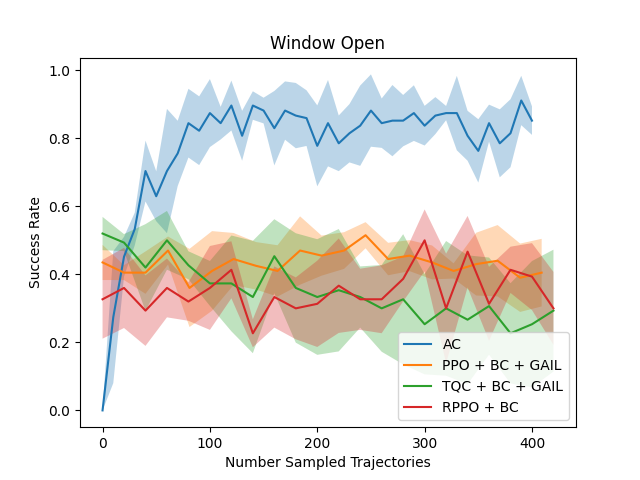
\includegraphics[width=\textwidth]{images/FineTuning/Window Open.png}
      \caption{Window Open environment, 4 expert demonstrations.}
      \label{fig:plot3}
    \end{subfigure}
    \begin{subfigure}[t]{0.45\textwidth}
      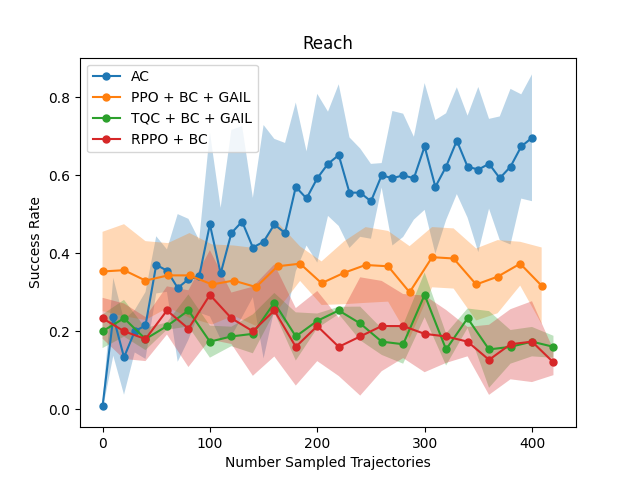
\includegraphics[width=\textwidth]{images/FineTuning/Reach.png}
      \caption{Reach environment, 4 expert demonstrations.}
      \label{fig:plot1}
    \end{subfigure}
    \medskip
    \begin{subfigure}[t]{0.45\textwidth}
      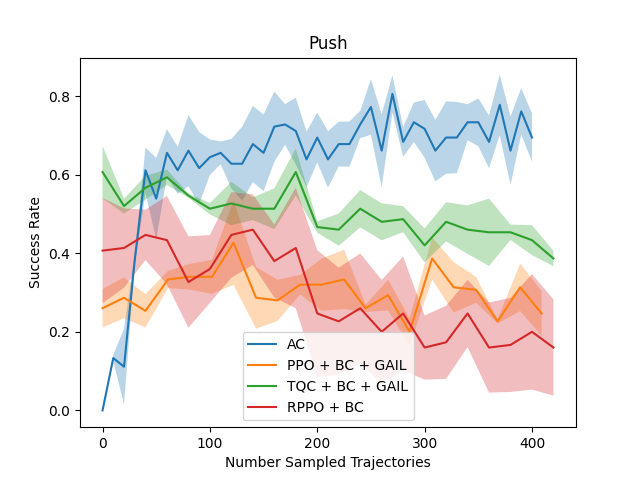
\includegraphics[width=\textwidth]{images/FineTuning/Push.png}
      \caption{Push environment, 15 expert demonstrations.}
      \label{fig:plot2}
    \end{subfigure}
    \begin{subfigure}[t]{0.45\textwidth}
      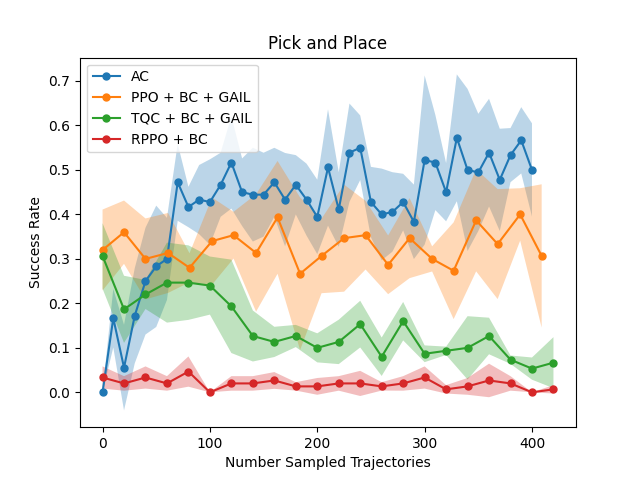
\includegraphics[width=\textwidth]{images/FineTuning/Pick and Place.png}
      \caption{Pick and Place environment, 15 expert demonstrations.}
      \label{fig:plot4}
    \end{subfigure}
    \caption{
    The learner trained by GAIL and RPPO were pretrained using behavioural cloning with the given number of expert demonstrations. 
    The x-axis shows the number of sampled environment epsiodes, each with 100 steps.  One initial observation and a sparse reward signal at the end of each episode was provided.}
    \label{fig:finetuning}
\end{figure}

\subsection{Guided Reinforcement Learning}
\label{sec:g_ref_ler}
In this section, we test the performance of AVC given minimal expert guidance. We use the "Reach" and "Window Open" environments with 2000 training episodes per run and three runs per experiment and learner.
Per data point, we sampled 30 trajectories to evaluate the success rate.\\
With this setting, the algorithms must learn most of the behavior from reinforcement learning, but the expert
demonstration is needed to overcome the initial search problem. We only provide sparse reward and one observation per trajectory, thus finding the first viable solution by unguided
trial and error is unviable for most problems. However, we found the "Drawer Close" environment can be learned without any expert guidance.\\
For the baselines, we used RPPO, PPO and TQC with behavioural cloning as pre-training, where expert trajectories are provided. The results
are shown in figure \ref{fig:guided_ref}.

\begin{figure}[htbp]
    \centering
    \begin{subfigure}[t]{0.32\textwidth}
      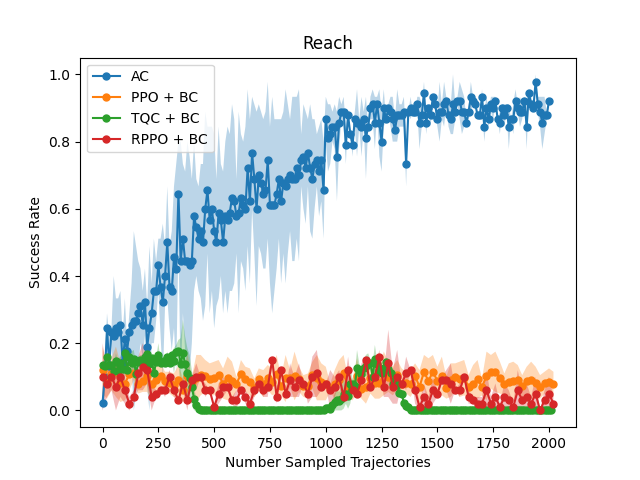
\includegraphics[width=\textwidth]{images/1_2000/Reach.png}
      \caption{1 expert demonstration.}
    \end{subfigure}
    \begin{subfigure}[t]{0.32\textwidth}
      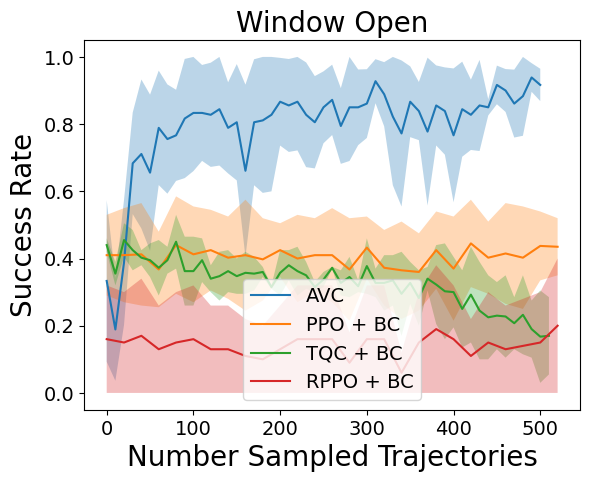
\includegraphics[width=\textwidth]{images/1_2000/Window Open.png}
      \caption{1 expert demonstration.}
    \end{subfigure}
    \begin{subfigure}[t]{0.32\textwidth}
      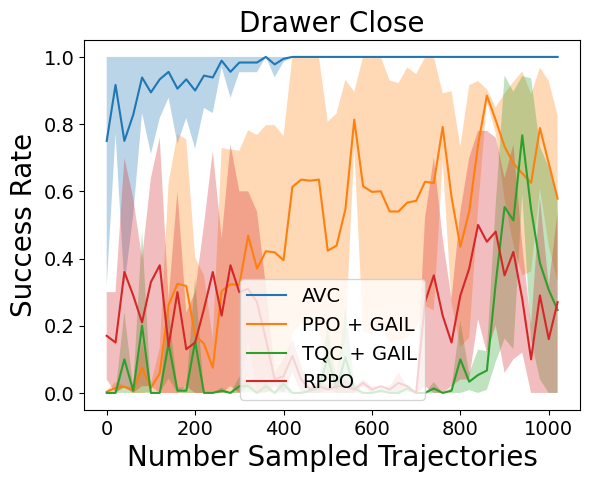
\includegraphics[width=\textwidth]{images/0/Drawer Close.png}
      \caption{0 expert demonstrations.}
      \label{fig:drawerclose}
    \end{subfigure}
    \medskip
    \begin{subfigure}[t]{0.45\textwidth}
      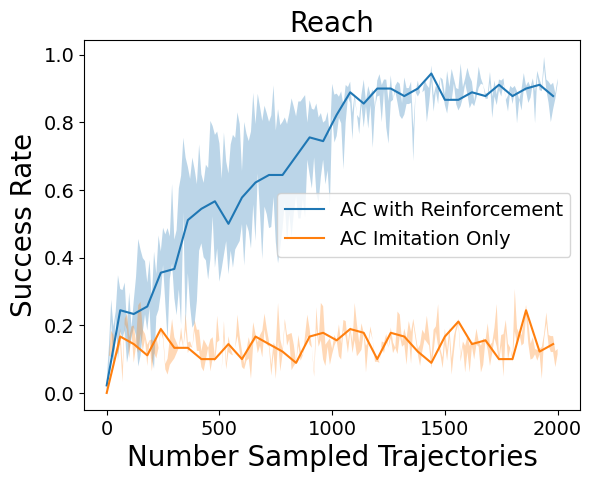
\includegraphics[width=\textwidth]{images/1_2000_imi/Reach.png}
      \caption{Reach environment. Comparison between pure imitation learning and reinforcement learning.}
    \end{subfigure}
    \hfill
    \begin{subfigure}[t]{0.45\textwidth}
      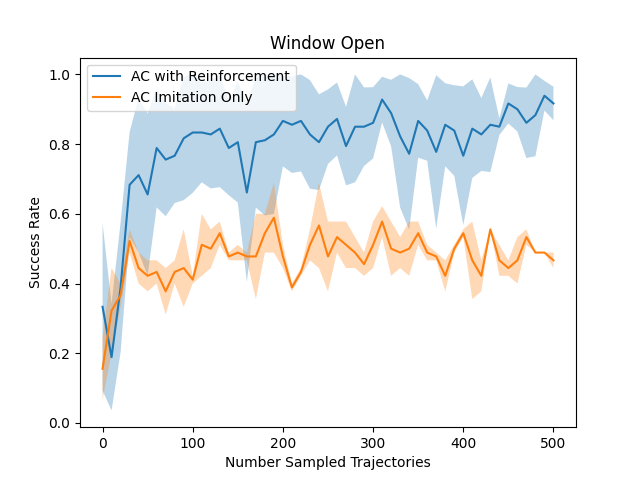
\includegraphics[width=\textwidth]{images/1_2000_imi/Window Open.png}
      \caption{Window Open environment. Comparison between pure imitation learning and reinforcement learning.}
    \end{subfigure}
    \caption{
    The learner trained by PPO, RPPO and TQC were pretrained using behavioural cloning given one demonstration except in the drawer close environment. 
    The pure imitation learning experiments on the buttom row were conducted using no additional epsiodes from the environment. There, the x-axis 
    displays equal amount of compute compared to the reinforcement learning runs.
    Each experiment was repeatet three times with 
    50 sampled validation episodes per run and data point. The shaded region displays one standard deviation.}
    \label{fig:guided_ref}
\end{figure}

The AVC algorithm was able to solve all environments with high success rates after 1000 or 2000 sampled trajectories. In "Reach" and "Window Open" the initial performance
of behavioural cloning was not improved in the reinforcement phase by any of the baselines. Similar to our discussion in section \ref{sec:fine_tuning},
we had to choose small learning rates to prevent catastrophic forgetting. With higher learning rates, all algorithms dropped to $0 \%$ success rate and did
not recover in initial tests. We find from the experiments that the challenging one observation sparse reward environment is difficult to learn in for
traditional actor-critic algorithms. In these setups, AVC shows a significant improvement.\\

We wanted to rule out that the performance difference comes mainly from our behavioural cloning setup. As PPO and TQC natively don't make use of expert demonstrations,
we pretrained them using behavioural cloning. We expected that from the pretraining, at least one successful trajectory would be sampled in the training phase, thus
helping to overcome the initial search problem. We find that all algorithms perform significantly above $0\%$ success rate, so we conclude that all algorithms had
access to guidance to find successful trajectories. To further rule out that our methodology gives an unequal advantage to our algorithm, we tested all algorithms on the
"Drawer Close" environment. We found that random trajectories can already solve the environment with about $20\%$ success rate, so no expert guidance is needed to learn a feasible behaviour.
The results are shown in subfigure \ref{fig:drawerclose}. The difference in performance at 0 environment interactions comes from random initialization. As we only had time for three runs per
experiment, there is some noise in the data. However, all algorithms sample trajectories randomly in the initial training phase. We set the initial random phase to
1000 steps or 10 trajectories, so all algorithms had access to some successful trajectories with high probability. \\

From the plot, it can be seen that PPO steadily improves performance, which is expected, as on-policy algorithms tend to be more stable.
TQC learns rapidly in some sections but seems to overshoot and fall back to bad performance frequently.
We find it to be more dependent on hyperparameters than PPO and RPPO.
The high variance shown from the baselines in the plot can be explained by the sparse rewards, which provide highly nonlinear feedback.
AC rapidly improved to perfect performance within about 400 steps. \\

Next, we wanted to rule out that the observed performance gain of AVC over the baselines comes mostly from the different underlying neural network architectures. AVC uses transformers for the actor and
critic, while the TQC and PPO implementations use MLPs and the RPPO implementation uses a GRU. To do this, we tested the performance of AVC using pure imitation learning shown on the bottom row of
figure \ref{fig:guided_ref}. We expect the main improvement of behavioural cloning in AC, TQC and PPO over a recurrent policy comes from the sequence encoding, as proposed in section \ref{COD_AC}.
We find that the pure imitation learning performance
of AVC is about the same as behavioural cloning for PPO and TQC. While in the Window Open environment, both PPO and TQC outperformed RPPO, we find that in the Reach environment RPPO performs
similar to PPO. As only one expert trajectory was provided and we repeated the experiment three times, we find the difference between RPPO, PPO and TQC in the Reach
environment too small to make conclusions about their relative performance, given the variance from the data. \\

Overall, we take this finding as evidence for the effectiveness of the AVC algorithm. It is highly unlikely that the observed improvement
over the baselines comes only from the transformer architecture underlying the AVC actor and critic, given the similar behavioural cloning performance. We also find clear improvement of AVC with
reinforcement learning over AVC with pure imitation learning, which demonstrates the AVC algorithm makes effective use from the additional feedback. 

\subsection{Comparison of Optimisation Modes}
\label{ref:com_opt_modes}
In section \ref{sec:inf_time_search} we discussed that we can use different modes of optimisation during inference time to optimize the action sequemce. In this section, 
we showcase the difference between optimizing the action sequence directly and optimizing the actor and planner weights. We tested the two different 
modes in the reach environment with the same setup as in section \ref{sec:g_ref_ler}, thus we used the same data for the actor planner optimisation runs. For the direct 
action optimisation runs we used 20000 sampled episodes to see, if reinforcement learning took place at all, as for the first 2000 epsiodes no improvement above 
imitation learning performance is seen. For this reason, we only repeated the experiment twice, as it took a long time to compute. The results are depicted in figure 
\ref{fig:action_vs_actor}. It is obvious, that the optimisation mode is key to the reinforcement learning perforance. We hypothesize a reason for the much 
faster convergence rate of the actor planner optimisation mode is, that they encode an informed representation of the space of useful trajectories with 
respect to the environment, which is guiding the search. Subfigure \ref{fig:direct_actions} shows the changes to the trajectory given the gradient from the critic is applied 
directly to the actions, while subfigure \ref{fig:ac_pl_actions} shows the changes given the gradient is applied to the actor and planner. We find 
subfigure \ref{fig:ac_pl_actions} shows a structured exploration, while subfigure \ref{fig:direct_actions} is more random. 

\begin{figure}[htbp]
    \centering
    \begin{subfigure}[t]{0.65\textwidth}
      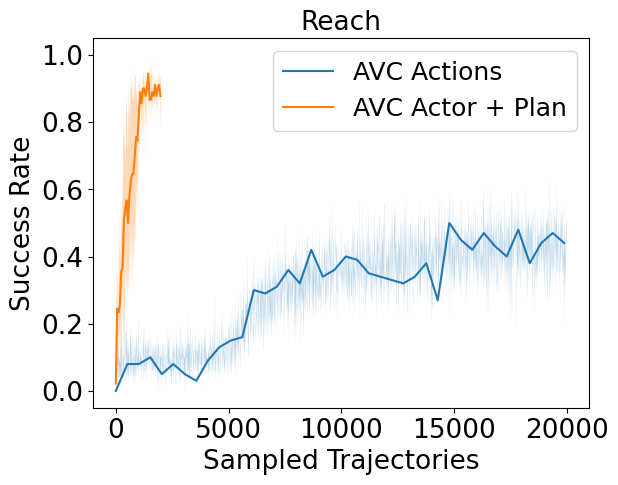
\includegraphics[width=\textwidth]{images/Plan_vs_Actions/Reach.png}
      \caption{Reach environment. Shown is the difference in learning efficiency of the Active Critic algorithm using two different optimisation modes.}
      \label{fig:plot1}
    \end{subfigure}
    \medskip
    \begin{subfigure}[t]{0.45\textwidth}
      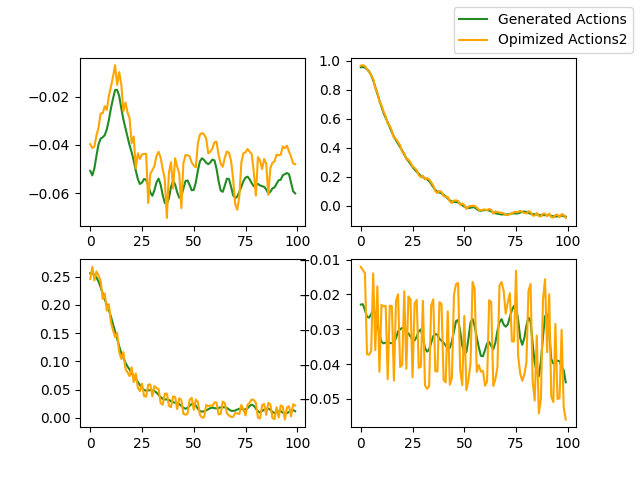
\includegraphics[width=\textwidth]{images/Plan_vs_Actions/changes/actions_1.png}
      \caption{Optimized trajectories (orange) and trajectories proposed by the actor (green). The gradient from the critic was applied to the actions.}
      \label{fig:direct_actions}
    \end{subfigure}
    \hfill
    \begin{subfigure}[t]{0.45\textwidth}
      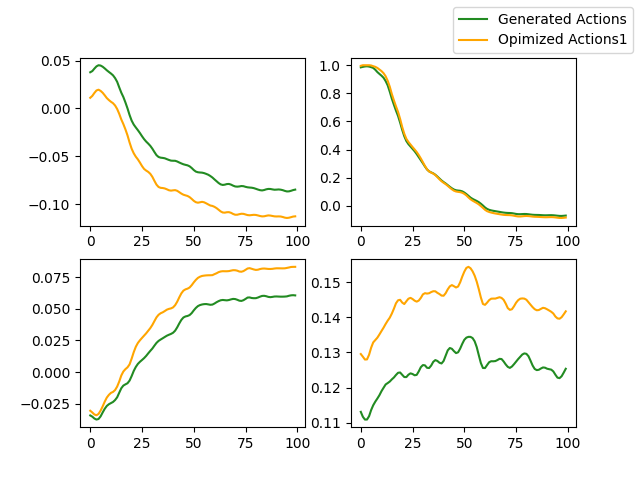
\includegraphics[width=\textwidth]{images/Plan_vs_Actions/changes/plans_actor_0.png}
      \caption{Optimized trajectories (orange) and trajectories proposed by the actor (green). The gradient from the critic was applied to the actor and planner.}
      \label{fig:ac_pl_actions}
    \end{subfigure}
    \caption{Comparison of two different optimisation modi. Each experiment was repeated twice with 30 evaluation episodes per data point.
    The x-axis shows the number of sampled environment epsiodes, each with 100 steps. One initial observation and a sparse reward signal at the end of each episode was provided.}
    \label{fig:action_vs_actor}
\end{figure}

\subsection{Dense Observations}
In this section we test the relaxation of the AVC algorithm to MDP environments, developed in section \ref{sec:relax_dense}, with the environment state given as an observation after each step. \\
We use sparse rewards 
and compare "Dense Observation Active Critic" (DOAC) to PPO and TQC on the "Reach", "Window Open" and "Drawer Close" environments. Again, we don't use "HER", as it limits the generality of 
the approach. Apart from 
providing an observation per time step,
we use the same setup as discribed in previous sections. The results are shown in figure \ref{fig:dense_ref}. First, we find that both base line algorithms 
start at similar perforance from behavioural cloning as in the single observation setup, which is expected, since behavioural cloning does not rely on 
environment interactions. After the first data point, both algorithms sharply drop to near zero perforance, which is worse perforance then for the single 
observation runs. We explain this with the distribution shift after training starts. Additionally to the overestimation by the critic, as discussed earlier, a policy trained by imitation learning 
will induce a different distribution of observations then the expert data. This breaks the i.i.d. assumption. In the single observation case for PPO and TQC, this assumption was not broken, 
as the inputs are the first observtion, which distribution is a constant of the environment. In the MDP setup with enviroment state observations, most input data is 
sampled according to the current policy and thus the i.i.d. assumption is broken. PPO did not find solutions to the "Reach" and "Window Open" environments, 
but we find TQC got about $20 \%$ success rate on "Reach" and achieved about $80 \%$ success rate on "Window Open" leveling out after about 2500 episodes. 
The superior perforance of TQC over PPO is expected, as TQC tends to perfrom better in environments where exploration is important. As TQC now gets 
feedback from it's actions on the environment, the better exploration is an advantage over PPO.\\ 
TQCs perforance drops to about $0 \%$ for the "Window Open" 
environment after the first data point showing the performance from behavioural cloning. We wanted to analyze, if TQC uses the guidance from the expert at all, or if it starts from 
no usable knowledge about the environment. To do this, we also conducted the experiment three times with no initial behavioural cloning. The results are shown in 
subfigure \ref{fig:TQC_0_vs_exp}. We find that TQC can solve the environment within 5000 steps from no expert demonstrations in one case, but does not find a good policy in the other two. 
We propose pretraining from behavioural cloning is a useful bias for the algorithm to find feasable solutions quicker with higher probability. Following this insight, 
we also conducted the "Window Open" experiment in MDP setting with GAIL to make better use of the provided expert demonstration. We find our initial 
baseline with pretrained TQC performs best. This is probably due to the fact that GAIL makes no use of the sparse reward. Additionaly, 
the authos mentioned in the paper, that GAIL is not more efficient in terms of environment interactions then TRPO with rewards. A large number of 
environment interactions is needed, before the discriminator of GAIL provides useful rewards for the learner. We suppose that is a reason, why GAIL does not perform 
well in our setting, where relatively small amount of environment interactions are used. \\

Overall, DOAC is the only algorithm that can greatly benefit from expert demonstration in the sparse reward setting and 
it significantly outperforms all baselines including additional tests with GAIL. \\

We also included results for the "Drawer Close" environment with no expert demonstrations. All algorithms perform better then in the single observation environment, 
but DOAC is the only algorithm with stable perforance. It found a solution with near perfect success rate in all three runs quickly. \\
Overall, DOAC performs well in all shown environments. Especially in the "Reach" environment it is the only algorithm that finds a feasable solution while it 
converges much quicker and has a more robust bahaviour in general. 

\begin{figure}[htbp]
  \centering
  \begin{subfigure}[t]{0.45\textwidth}
    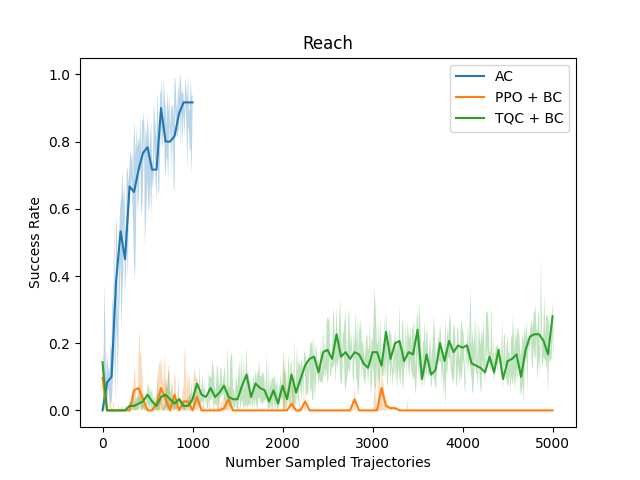
\includegraphics[width=\textwidth]{images/dense_1/Reach.png}
    \caption{One expert demonstration.}
  \end{subfigure}
  \hfill
  \begin{subfigure}[t]{0.45\textwidth}
    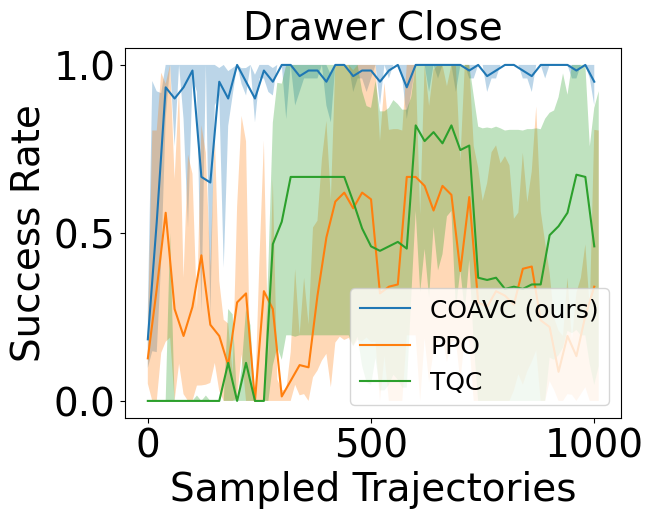
\includegraphics[width=\textwidth]{images/dense_0/Drawer Close.png}
    \caption{No expert demonstrations.}
  \end{subfigure}
  \medskip
  \begin{subfigure}[t]{0.45\textwidth}
    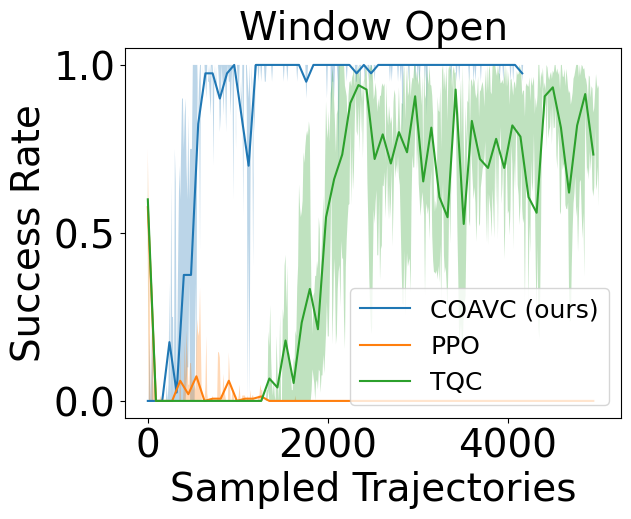
\includegraphics[width=\textwidth]{images/dense_1/Window Open.png}
    \caption{One expert demonstration.}
  \end{subfigure}
  \hfill
  \begin{subfigure}[t]{0.45\textwidth}
    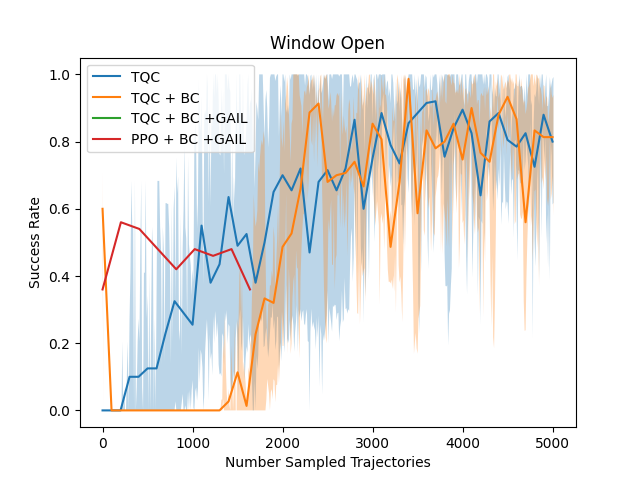
\includegraphics[width=\textwidth]{images/TQC_bc_GAIL_vs_ref/Window Open.png}
    \caption{Comparison between TQC with no expert demonstrations and expert guided baselines.}
    \label{fig:TQC_0_vs_exp}
  \end{subfigure}
  \caption{Comparison between DOAC and various baselines given one or no expert demonstrations. The environment state was provided after each step.
  Each experiment was repeated three times with 50 evaluation episodes per data point.}
  \label{fig:dense_ref}
\end{figure}

\subsection{Comparison of Dense and Single Observation}
In this section we compare DOAC and AC, to investigate if DOAC makes use of the additionally provided information. The results are shown in figure \ref{fig:dense_vs_single}.
We find that in "Reach" and "Drawer Close", DOAC converges quicker. Especially in "Reach", we see a stable improvement from DOAC over AC. In "Drawer Close", the difference is 
small, which is mainly due to the fact that AVC already solves the environment very quickly. Note hoever, that DOAC had worse initial perforance then AVC in the shown experiments. 
As we discussed earlier, the initial perforance comes from the random initialisation and varies greatly. We take the fact that DOAC converged quicker then AVC even though it had 
worse starting initialisations in the three runs as further evidence, that DOAC makes effective use of the additional information. In the "Window Open" environment, DOAC initially converged slower but 
reached near pefect performance quicker then AC. We suppose this is due to the different optimisation modes used for the two algorithms. Recall that AVC optimizes the whole 
trajectory at the beginning, while DOAC makes small improvements per time step, due to self imposed inference time constraints. We expect this has the effect that in inference time, the critic of 
AC can make larger changes to the trajectory proposed by the actor. In other words, while the actor converges DOAC makes smaller moves towards the critic target then AC. Also out of time constraints, we could 
not conduct a hyper parameter search for DOAC. It is possible that DOAC would converge quicker, given more optimisation steps per inference step or a higher inference optimisation 
learning rate $\alpha_{inf}$.\\ 
AC already performs close to the MDP setup used by DOAC. We propose this is due to the fact, that AVC uses the information about the environment 
from the expert demonstrations effectively to search for new candidate solutions. As discussed in section \ref{ref:com_opt_modes}, AVC searches on a preimposed subspace given the "knowledge" of the 
actor. This means it does not conduct random search even though it does not not get any feedback from the environment. This is probably a key for the good perforance of AVC and DOAC and explains 
the relative close perforance of both algorithms. We expect a major advantage of DOAC over AVC in non deterministic environments, as AVC sould not be able to solve those from the initial 
observation alone. DOAC already has a method to disambiguate action sequences given the same observations as discussed in section \ref{avr_action_problem}, which is key, if the same initial 
observations and actions can lead to different observations at later time steps. However out of time constraints, we leave this research question to future work.\\
Overall we find that DOAC works well in the tested environments and outperforms all baselines in the MDP setting with sparse rewads.

\begin{figure}[htbp]
  \centering
  \begin{subfigure}[t]{0.32\textwidth}
    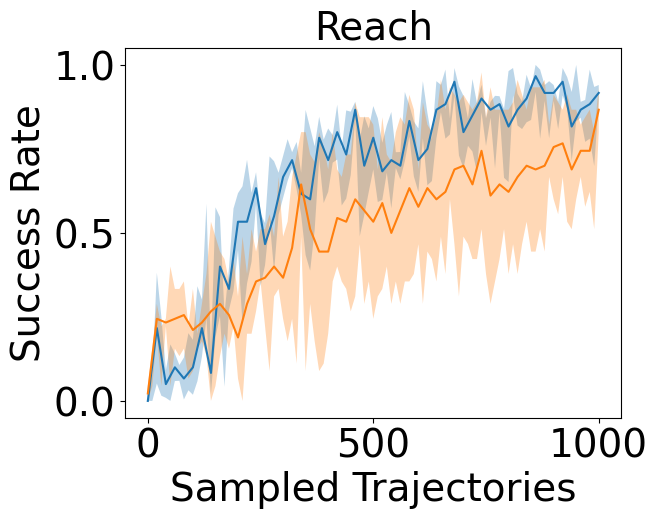
\includegraphics[width=\textwidth]{images/dense_vs_sparse_1/Reach.png}
    \caption{1 expert demonstration.}
  \end{subfigure}
  \medskip
  \begin{subfigure}[t]{0.32\textwidth}
    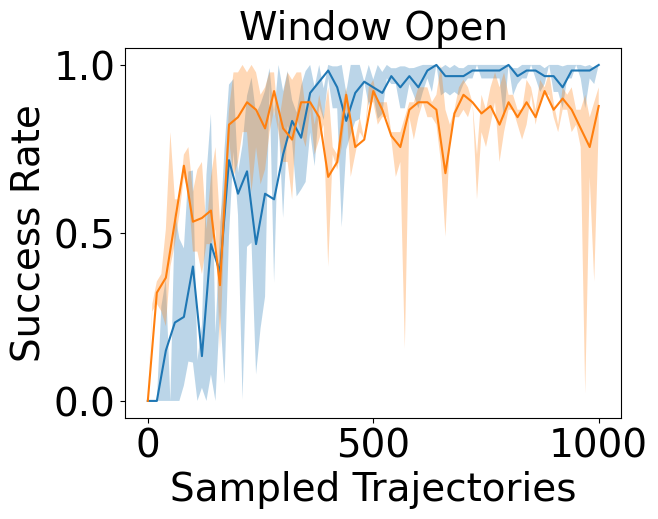
\includegraphics[width=\textwidth]{images/dense_vs_sparse_1/Window Open.png}
    \caption{1 expert demonstration.}
  \end{subfigure}
  \hfill
  \begin{subfigure}[t]{0.32\textwidth}
    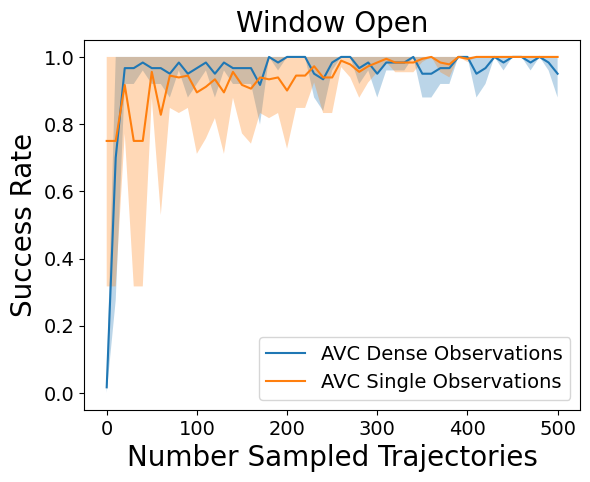
\includegraphics[width=\textwidth]{images/dense_vs_sparse_0/Window Open.png}
    \caption{0 expert demonstrations.}
  \end{subfigure}
  \caption{Comparison of AVC in single observation and DOAC in mdp environments. Each experiment was repeated three times with 50 evaluation episodes per data point.
  }
  \label{fig:dense_vs_single}
\end{figure}